%%%%%%%%%%%%%%%%%%%%%%%%%
% Dokumentinformationen %
%%%%%%%%%%%%%%%%%%%%%%%%%
% !TeX program = pdflatex
% !TeX encoding = utf8
% !TeX spellcheck = de_DE
\newcommand{\titleinfo}{Nice to Know}
\newcommand{\authorname}{\href{mailto:mgisler@hsr.ch}{M. Gisler} }
\newcommand{\authoremail}{\href{mailto:mgisler@hsr.ch}{M. Gisler} }

%BuG-Fix
%Package pdf Error: Driver file ................ not found
%If you have a luatex driver fail uncomment these lines
\RequirePackage{luatex85}
\def\pgfsysdriver{pgfsys-pdftex.def}
% Genereller Header
\documentclass[11pt,twoside,a4paper,fleqn]{article}
% Dateiencoding
%\usepackage{fontspec}
%\setmainfont{Calibri}
\usepackage[utf8]{inputenc}
\usepackage[T1]{fontenc}	%ä,ü...
% Seitenränder
\usepackage[left=1cm,right=1cm,top=0.5cm,bottom=0.5cm,includeheadfoot]{geometry}
% Sprachpaket
\usepackage[ngerman]{babel} % Silbentrennung und Rechtschreibung Englisch und Deutsch

%%%%%%%%%%%%%%%%%%%%%%%
%% Wichtige Packages %%
%%%%%%%%%%%%%%%%%%%%%%%
\usepackage{amsmath}                % Allgemeine Matheumgebungen									
\usepackage{amssymb}                % Fonts: msam,msbm, eufm & Mathesymbole, Mengen (lädt automatisch amsfonts)									
\usepackage{array}                  % \newcolumntype, \firsthline, ,\lasthline, m{width}, b{width}									
\usepackage{caption}                % Bildunterschriften									
\usepackage{enumitem}               % basic environments: enumerate, itemize, description									
\usepackage{fancybox}               % \fbox: \shad­ow­box, \dou­ble­box, \oval­box, \Oval­box									
\usepackage{fancyhdr}               % Seiten schöner gestalten, insbesondere Kopf- und Fußzeile									
\usepackage{floatflt}               % Textumflossene Abbildungen \begin{floatingfigure}[r]{Breite} : r rechts, l links, p links auf geraden Seiten und rechts auf ungeraden Seiten									
\usepackage{graphicx}               % \includegraphics[keyvals]{imagefile}, [draft]graphicx zeigt nur Namen und Rahmen an, [final] hebt diese option auf => Bild wird angezeigt    									
\usepackage{hyperref}               % Erstellt Verweise innerhalb und nach außerhalb eines PDF Dokumentes.									
\usepackage{lastpage}               % Bspw. : Page 1 of 3 => \thepage\ of \pageref{LastPage}									
\usepackage{listings}               % Erlaubt es Programmcode in der gewünschten Sprache zu hinterlegen (C++, Matlab,..). Definition der Sprache mit \lstset{language=name}..									
\usepackage{longtable}              % Longtable erlaubt es Tabellen zu erstellen die bei der nächsten Seite weiterlaufen. (Bricht automatisch um)									
\usepackage{mathabx}                % Mathesymbole									
\usepackage{mathrsfs}               % \mathscr (Benötigt für Fourierreihen-Symbol)									
%\usepackage{mathtools}              % Extension package to amsmath									
\usepackage{multicol}               % multicols-Umgebung \begin{multicols}{3} erzeugt Abschnitt mit 3 Spalten									
\usepackage{multirow}               % Tabelle: ermöglicht es Felder mehrerer Zeilen in einem zusammenzufassen									
\usepackage{pdflscape}              % adds PDF support to the environment 'landscape'									
\usepackage{pxfonts}                % Symbole, griechisches Alphabet, Integrale...									
\usepackage{rotating}               % sideways, turn{degree}, rotate{degree}, sidewaysfigure, sidewaystable Umgebung									
\usepackage{subcaption}             % Bildunterschriften für Subfigures									
\usepackage{tabularx}               % tabularx-Umgebung: Hat feste Gesamtbreite, \begin{tabularx}{\textwidth}{c c c c c} X: Spalte mit variabler Breite, l, c, r, p{breite}, m{breite}									
\usepackage{textcomp}               % text symbols: baht, bullet, copyright, musical-note, onequarter, section, yen									
\usepackage{tikz}                   % Tikz Umgebung zur Grafikerzeugung									
\usepackage{titlesec}               % Überschriften zu Textabstände
\usepackage{trfsigns}               % Transformationszeichen \laplace, \Laplace..									
\usepackage{trsym}                  % Weitere Laplace Zeichen erlaubt auch vertikale Transformationszeichen									
\usepackage{verbatim}               % verbatim, verbatim*, comment Umgebung									
\usepackage{wrapfig}                % Textumflossene Bilder und Tabellen, \begin{wrapfigure}[Zeilen]{Position}[Ueberhang]{Breite}									
\usepackage{xcolor}                 % \pagecolor{color}, \textcolor{color}{text}, \colorbox{color}{text}, \fcolorbox{border-color}{fill-color}{text}									
\usepackage{titlesec}
% Zum Bilder einfach in Tabellen einfügen (valign=t)
\usepackage[none]{hyphenat}
\usepackage[export]{adjustbox}
\usepackage{circuitikz}
\usetikzlibrary{decorations.markings,arrows}
\usepackage{esint}
\usepackage{graphics}
\usepackage{pdfpages} 

%%%%%%%%%%%%%%%%%%%%
% Generelle Makros %
%%%%%%%%%%%%%%%%%%%%


\newcommand\tabbild[2][]{%
	\raisebox{0pt}[\dimexpr\totalheight+\dp\strutbox\relax][\dp\strutbox]{%
		\includegraphics[#1]{#2}%
	}%
}


%%%%%%%%%%
% Farben %
%%%%%%%%%%
\definecolor{black}{rgb}{0,0,0}
\definecolor{red}{rgb}{1,0,0}
\definecolor{white}{rgb}{1,1,1}
\definecolor{grey}{rgb}{0.8,0.8,0.8}
\definecolor{green}{rgb}{0,.8,0.05}
\definecolor{brown}{rgb}{0.603,0,0}
\definecolor{mymauve}{rgb}{0.58,0,0.82}


%%%%%%%%%%%%%%%%%%%%%%%%%%%%
% Mathematische Operatoren %
%%%%%%%%%%%%%%%%%%%%%%%%%%%%
\DeclareMathOperator{\sinc}{sinc}
\DeclareMathOperator{\sgn}{sgn}
\DeclareMathOperator{\Real}{Re}
\DeclareMathOperator{\Imag}{Im}
\DeclareMathOperator{\euler}{e}
\DeclareMathOperator{\cov}{cov}
\DeclareMathOperator{\PolyGrad}{PolyGrad}
\DeclareMathOperator{\gradient}{grad}
\DeclareMathOperator{\rotation}{rot}
\DeclareMathOperator{\divergenz}{div}
\DeclareMathOperator{\imaginär}{j}
\DeclareMathOperator\arccot{arccot}
\DeclareMathOperator\arcsec{arcsec}
\DeclareMathOperator\arcossec{arcossec}
\DeclareMathOperator\arsinh{arsinh}
\DeclareMathOperator\arcosh{arscosh}
\DeclareMathOperator\artanh{artanh}
\DeclareMathOperator\arcoth{arcoth}


%%%%%%%%%%%%%%%%%%%%%%%%%%%%
% Allgemeine Einstellungen %
%%%%%%%%%%%%%%%%%%%%%%%%%%%%
%Pdf Info
\hypersetup{pdfauthor={\authorname},pdftitle={\titleinfo},colorlinks=false}
\author{\authorname}
\title{\titleinfo}


%%%%%%%%%%%%%%%%%%%%%%%
% Kopf- und Fusszeile %
%%%%%%%%%%%%%%%%%%%%%%%
\pagestyle{fancy}
\fancyhf{}
%Linien oben und unten
\renewcommand{\headrulewidth}{0.5pt} 
\renewcommand{\footrulewidth}{0.5pt}

%Kopfzeile links bzw innen
\fancyhead[L]{\titleinfo{ }}
%Kopfzeile mitte
%\fancyhead[C]{}
%Kopfzeile rechts bzw. aussen
\fancyhead[R]{Seite \thepage { }von \pageref{LastPage}}

%Fusszeile links bzw. innen
\fancyfoot[L]{\footnotesize{\authorname}}
%Fusszeile mitte
\fancyfoot[C]{\footnotesize{Elektrotechnik@HSR}}
%Fusszeile rechts bzw. ausen
\fancyfoot[R]{\footnotesize{\today}}
% Einrücken verhindern versuchen
\setlength{\parindent}{0pt}



%%%%%%%%%%%%%%%%%%%%%%%%%%
%	Dokument			%%
%%%%%%%%%%%%%%%%%%%%%%%%%%
\begin{document}
\title{\Huge{Nice to Know}}
\maketitle
Zusammenstellung von Sachen, welche immer wieder gebraucht werden

\tableofcontents
\setcounter{tocdepth}{2} %Setzt tiefe des Inhaltsverzeichnis
\thispagestyle{empty}
\newpage
\input{sections/siEinheiten}
\input{sections/griechischesAlphabet}
\section{Rechengesetze}
\begin{multicols}{2}
\subsection{Potenzregeln}
\renewcommand{\arraystretch}{2}
\begin{tabular}{|c|c|}
	\hline $a^0=1$ & $a^-n= \frac{1}{a^n}$\\
	\hline $a^m \cdot a^n = a^m+n$ & $\frac{a^n}{a^m}= a^n-m$\\
	\hline $(a^n)^m = a^n*m$ & $(\frac{a}{b})^n = \frac{a^n}{b^n}$\\
	 \hline $a^n*b^n = (ab)^n$ & $a^\frac{b}{n}= \sqrt[n]{a^b}$\\
	 \hline
\end{tabular}

\subsection{Wurzelregeln}
\renewcommand{\arraystretch}{2}
\begin{tabular}{|c|c|}
	\hline $\sqrt[n]{a^n}= (\sqrt[n]{a})^n$ & $\sqrt[n]{\frac{a}{b}} = \frac{\sqrt[n]{a}}{\sqrt[n]{b}}$\\
	\hline $\sqrt[n]{a^x}=(\sqrt[n]{a})^x$ & $a\sqrt[n]{x} + b \sqrt[n]{x} = (a+b)\sqrt[n]{x}$\\
	\hline $\sqrt[n]{a \cdot b} = \sqrt[n]{a} \cdot \sqrt[n]{b}$ & $a\sqrt[n]{x} - b \sqrt[n]{x} = (a-b)\sqrt[n]{x}$\\
	\hline $\sqrt[n]{\sqrt[m]{a}}= \sqrt[n \cdot m]{a}$ & $\sqrt[n]{a^x}= a^\frac{x}{n}$ \\
	\hline
\end{tabular}
\end{multicols}

\subsection{Logarithmusregeln}
\begin{minipage}{10cm}
	\begin{tabbing}
		xxxxxxxxxxxxxxxx \= xxxxxxxxxxxxxxxx \= \kill
		$lg(x) = \log_{10} x$ \> $ln(x) = \log_{e} x$ \> $lb(x) = \log_{2} x$
	\end{tabbing}
	\renewcommand{\arraystretch}{2}
	\begin{tabular}{|c|c|}
		\hline $\log{xy} = \log{x} + log{y}$ & $\log{\sqrt[n]{x}}=\log{x^\frac{1}{n}}$\\
		\hline $\log{\frac{x}{y}}= \log{x} + log{y}$ & $\log{x^y}= y\log{x}$ \\
		\hline $\log{\sqrt[n]{x}}= \frac{\log{x}}{n}$ & $\log{1}=0$\\
		\hline
	\end{tabular}
\end{minipage}
\begin{minipage}{5cm}
	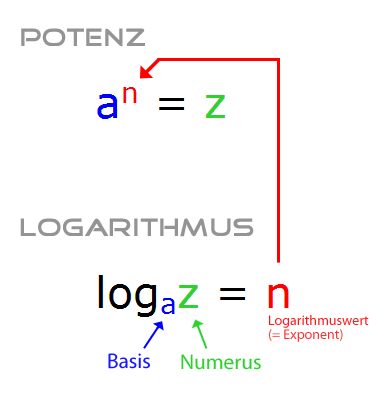
\includegraphics[width=4cm]{images/potenz_logarithmus.png}	
\end{minipage}

\begin{multicols}{2}
	\subsection{Binom}
	\renewcommand{\arraystretch}{2}
	\begin{tabular}{|c|}
		\hline $a^2+2ab+b^2 = (a+b)(a+b)$\\
		\hline $a^2-2ab+b^2 = (a-b)(a-b)$\\
		\hline $a^2-b^2= (a+b)(a-b)$\\
		\hline $(a \pm b)^3 =a^3 \pm  3 a^{2} b + 3 a b^2 \pm b^3 $\\
		\hline $(a \pm b)^4 =a^4 \pm  4 a^{3} b + 6a^2b^2 \pm 4 a b^3 +	b^4$\\
		\hline
	\end{tabular}
	
	\subsection{Quadratische Gleichung}
	\begin{tabbing}
		xxxxxxxxxxxxxxxxxxxx \= \kill
		$ax^2+bx+c=0$ \> $x_{1,2} = \dfrac{-b \pm \sqrt{b^2 - 4ac}}{2a}$
	\end{tabbing}
\end{multicols}

\subsection{Partialbruchzerlegung}
\[f(x)=\frac{x^2+20x+149}{x^3+4x^2-11x-30} \Rightarrow \; \begin{array}{l}\text{Nenner faktorisieren}
\end{array} \Rightarrow
x^{3}+4x^{2}-11x-30=(x+2)(x^{2}+2x-15)=(x+2)(x+5)(x-3)\] Ansatz:
\[f(x)=\frac{x^2+20x+149}{x^3+4x^2-11x-30}=\frac{A}{x-3} + \frac{B}{x+2} + \frac{C}{x+5}=
\frac{A(x+2)(x+5)+B(x-3)(x+5)+C(x-3)(x+2)}{(x-3)(x+2)(x+5)}\]
Gleichungssystem aufstellen mit beliebigen $x_i$-Werten (am Besten Polstellen oder 0,1,-1 wählen):
\[\begin{array}{l}x_1=3:\;-9+60+149=A\cdot5\cdot8\;\;\;\Rightarrow A=5\\
x_2=-2:\;-4-40+149=B(-5)\cdot3\; \Rightarrow B=-7\\
x_3=-5:\;-25-100+149=C(-8)(-3) \Rightarrow C=1 \end{array} \Rightarrow
f(x)=\frac{5}{x-3}-\frac{7}{x+2}+\frac{1}{x+5}\] weitere Ansätze für andere
Typen von Termen: \[f(x)=\frac{5x^2-37x+54}{x^3-6x^2+9x}=\frac{A}{x}+\frac{B}{x-3}+\frac{C}{(x-3)^2}=\frac{A(x-3)^2+Bx(x-3)+Cx}{x(x-3)^2}\]
\[f(x)=\frac{1,5x}{x^3-6x^2+12x-8}=\frac{A}{x-2}+\frac{B}{(x-2)^2}+\frac{C}{(x-2)^3}=\frac{A(x-2)^2+B(x-2)+C}{(x-2)^3}\]
\[f(x)=\frac{x^2-1}{x^3+2x^2-2x-12}=\frac{A}{x-2}+\frac{Bx+C}{x^2+4x+6}=\frac{A(x^2+4x+6)+(Bx+C)(x-2)}{(x-2)(x^2+4x+6)}\]


Variante mit Koeffizientenvergleich: \\
\begin{minipage}{9cm}
	\[F(s) = \frac{1}{s(s^2+6s+13)} = \frac{A}{s} + \frac{Bs+C}{s^2+6s+13}\]
	\[1 = A(s^2+6s+13) + s(Bs+C)\] 
	\[1 = s^2(A+B) + s(C+6A) + 13A\] 
	\[\Rightarrow 1 = 13A; (A+B)=0; (C+6A)=0\]
	\[\Rightarrow A=\frac{1}{13}; B=-\frac{1}{13}; C=-\frac{6}{13}\]
\end{minipage}
\begin{minipage}{9cm}
	$s^2: A+B = 0$\\
	$s^1: 6A+C =0$\\
	$s^0: 13A = 1$
\end{minipage}

\subsection{Hornerschema}
\begin{minipage}[t]{9cm}
	- Pfeile $\Rightarrow$ Multiplikation\\
	- Zahlen pro Spalte werden addiert\\
	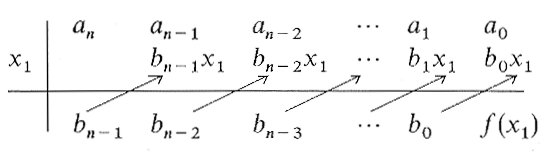
\includegraphics[width=6cm]{images/hornerschema_1.png}\\
	$x_1 \Rightarrow$ Nullstelle (muss erraten werden!!)\\
	oberste Zeile = zu zerlegendes Polynom			
\end{minipage}
\begin{minipage}[t]{9cm}
	\textbf{Beispiel:}\\
	$f(x) = x^3-67x-126$\\
	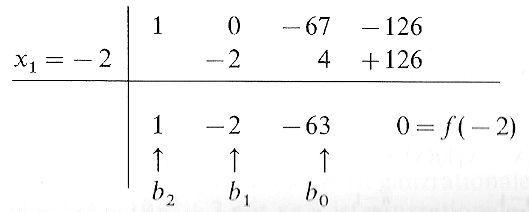
\includegraphics[width=6cm]{images/hornerschema_2.png}\\
	$\Rightarrow f(x) = (x-x_1)(b_2x^2 + b_1x + b_0) = (x+2)(x^2-2x-63)$	
\end{minipage}
\subsection{Winkelmasse}
\begin{tabular}{|l|l|l|}
	\hline & \textbf{Gradmass} & \textbf{Bogenmass}\\
	\hline \textbf{Einheit}& Grad, ° & Radiant, rad\\
	\hline \textbf{Vollwinkel}&  360° & 2$\pi$ rad\\
	\hline \textbf{Umrechnung} & $°= \frac{360}{2\pi} \cdot rad$ & $rad= \frac{2\pi}{360} \cdot °$\\
	\hline
\end{tabular}
\newpage
\input{sections/geometrischeGesetze}
\input{sections/komplexeZahlen}
\section{Trigonometrie}
\subsection{Winkelargumente}
\renewcommand{\arraystretch}{1.5}
\begin{tabular}{|c|c|c|c|c|c|c|c|c|c|c|c|c|c|c|c|c|c|c|c|c|}
	\hline \textbf{deg °} & $0$& $30$& $45$& $60$ &$90$&$120$& $135$&$150$&$180$ &$210$&$225$&$240$&$270$&$300$&$315$&$330$\\
	\hline \textbf{rad} & $0$& $\frac{\pi}{6}$&$\frac{\pi}{4}$&$\frac{\pi}{3}$&$\frac{\pi}{2}$&$\frac{2\pi}{3}$&$\frac{3\pi}{4}$&$\frac{5\pi}{6}$ &$\pi$&$\frac{7\pi}{6}$&$\frac{5\pi}{4}$&$\frac{4\pi}{3}$&$\frac{3\pi}{2}$&$\frac{5\pi}{3}$&$\frac{7\pi}{4}$&$\frac{11\pi}{6}$\\ 
	\hline \textbf{sin}&$0$&$\frac{1}{2}$&$\frac{\sqrt{2}}{2}$&$\frac{\sqrt{3}}{2}$&$1$&$\frac{\sqrt{3}}{2}$& $\frac{\sqrt{2}}{2}$&	$\frac{1}{2}$&$0$&$-\frac{1}{2}$ &$-\frac{\sqrt{2}}{2}$ &$-\frac{\sqrt{3}}{2}$ &$-1$&$-\frac{\sqrt{3}}{2}$ &$-\frac{\sqrt{2}}{2}$&$-\frac{1}{2}$\\
	\hline \textbf{cos}&$1$&$\frac{\sqrt{3}}{2}$ &$\frac{\sqrt{2}}{2}$&$\frac{1}{2}$ &$0$&$-\frac{1}{2}$&$-\frac{\sqrt{2}}{2}$&$-\frac{\sqrt{3}}{2}$&$-1$&$-\frac{\sqrt{3}}{2}$&$-\frac{\sqrt{2}}{2}$& $-\frac{1}{2}$&$0$&$\frac{1}{2}$&$\frac{\sqrt{2}}{2}$&$\frac{\sqrt{3}}{2}$\\
	\hline
\end{tabular}

\begin{multicols}{2}
	\subsection{Additionstheoreme}
	$\sin(a \pm b)=\sin(a) \cdot \cos(b) \pm \cos(a) \cdot \sin(b)$\\
	$\cos(a \pm b)=\cos(a) \cdot \cos(b) \mp \sin(a) \cdot \sin(b)$\\	
	$\tan(a \pm b)=\dfrac{\tan(a) \pm \tan(b)}{1 \mp \tan(a) \cdot \tan(b)}$
	
	\subsection{Doppel- und Halbwinkel}	
	$\sin(2a)=2\sin(a)\cos(a)$\\
	$\cos(2a)=\cos^2(a)-\sin^2(a)$\\
	$\cos^2 \left(\frac{a}{2}\right)=\frac{1+\cos(a)}{2} \qquad
	\sin^2 \left(\dfrac{a}{2}\right)=\frac{1-\cos(a)}{2}$

	\subsection{Produkte}
	$\sin(a)\sin(b)=\frac{1}{2}(\cos(a-b)-\cos(a+b))$\\
	$\cos(a)\cos(b)=\frac{1}{2}(\cos(a-b)+\cos(a+b))$\\
	$\sin(a)\cos(b)=\frac{1}{2}(\sin(a-b)+\sin(a+b))$\\	
	
	\subsection{Summe und Differenz}
	$\sin(a)+\sin(b)=2 \cdot \sin \left(\frac{a+b}{2}\right) \cdot
	\cos\left(\frac{a-b}{2}\right)$\\
	$\sin(a)-\sin(b)=2 \cdot \sin \left(\frac{a-b}{2}\right) \cdot
	\cos\left(\frac{a+b}{2}\right)$\\
	$\cos(a)+\cos(b)=2 \cdot \cos \left(\frac{a+b}{2}\right) \cdot
	\cos\left(\frac{a-b}{2}\right)$\\
	$\cos(a)-\cos(b)=-2 \cdot \sin \left(\frac{a+b}{2}\right) \cdot
	\sin\left(\frac{a-b}{2}\right)$\\
	$\tan(a) \pm \tan(b)=\dfrac{\sin(a \pm b)}{\cos(a)\cos(b)}$\\
	
	\subsection{Potenzen}
	$\sin^2(a)+\cos^2(a)=1$\\
	$\sin^2(a)-\cos^2(a)=1-2\sin^2(a)$\\
	$\sin^2(a)=\frac{1}{2}(1-\cos(2a))$\\
	$\cos^2(a)=\frac{1}{2}(1+\cos(2a))$\\
	$\sin^3(a)=\frac{1}{4}(3\sin(a)-\sin(3a))$\\
	$\cos^3(a)=\frac{1}{4}(3\cos(a)-\cos(3a))$\\
\end{multicols}

\subsection{Quadrantenbeziehungen}
\begin{tabbing}
	xxxxxxxxxxxxxxxxxxxxxxxxxxxxxxxxxx \= \kill
	$\sin(-a)=-\sin(a)$ \> $\cos(-a)=\cos(a)$\\
	$\sin(\pi - a)=\sin(a)$ \> $\cos(\pi - a)=-\cos(a)$\\
	$\sin(\pi + a)=-\sin(a)$ \> $\cos(\pi +a)=-\cos(a)$\\
	$\sin\left(\frac{\pi}{2}-a \right)=\sin\left(\frac{\pi}{2}+a \right)=\cos(a)$ \>
	$\cos\left(\frac{\pi}{2}-a \right)=-\cos\left(\frac{\pi}{2}+a \right)=\sin(a)$  
\end{tabbing}

\subsection{Plots}
\begin{multicols}{3}
	\subsubsection{Sinus-Funktion}
	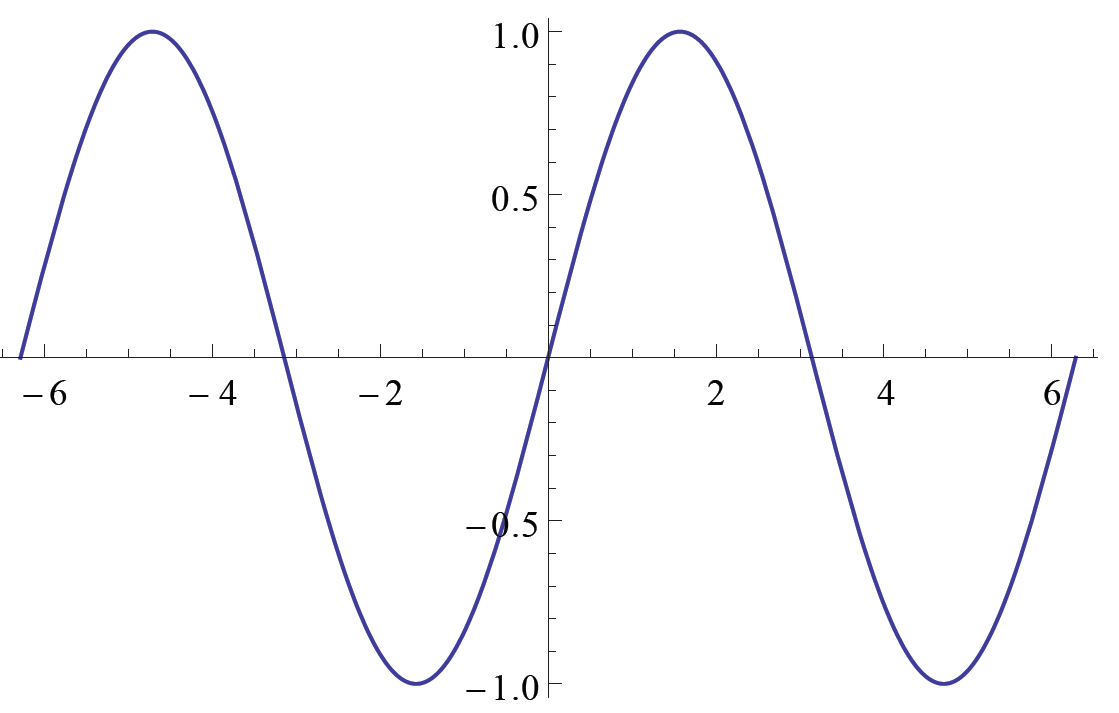
\includegraphics[width=5.5cm]{images/sin.png}
	\subsubsection{Cosinus-Funktion}
	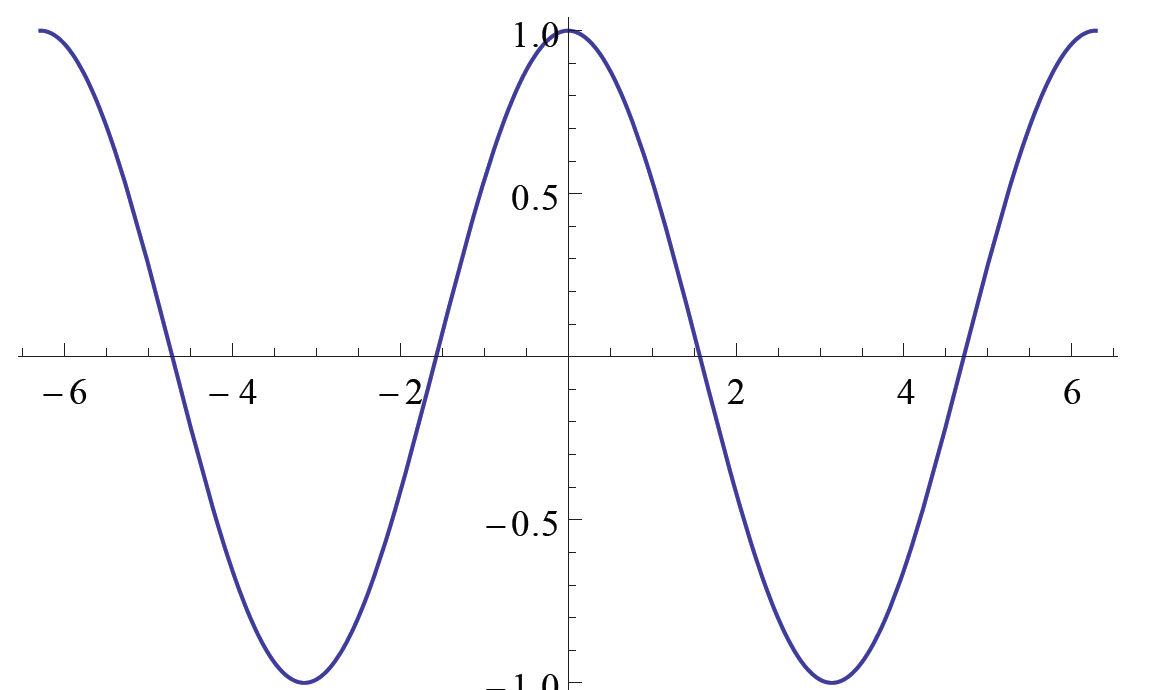
\includegraphics[width=5.5cm]{images/cos.png}
	\subsubsection{Tangens-Funktion}
	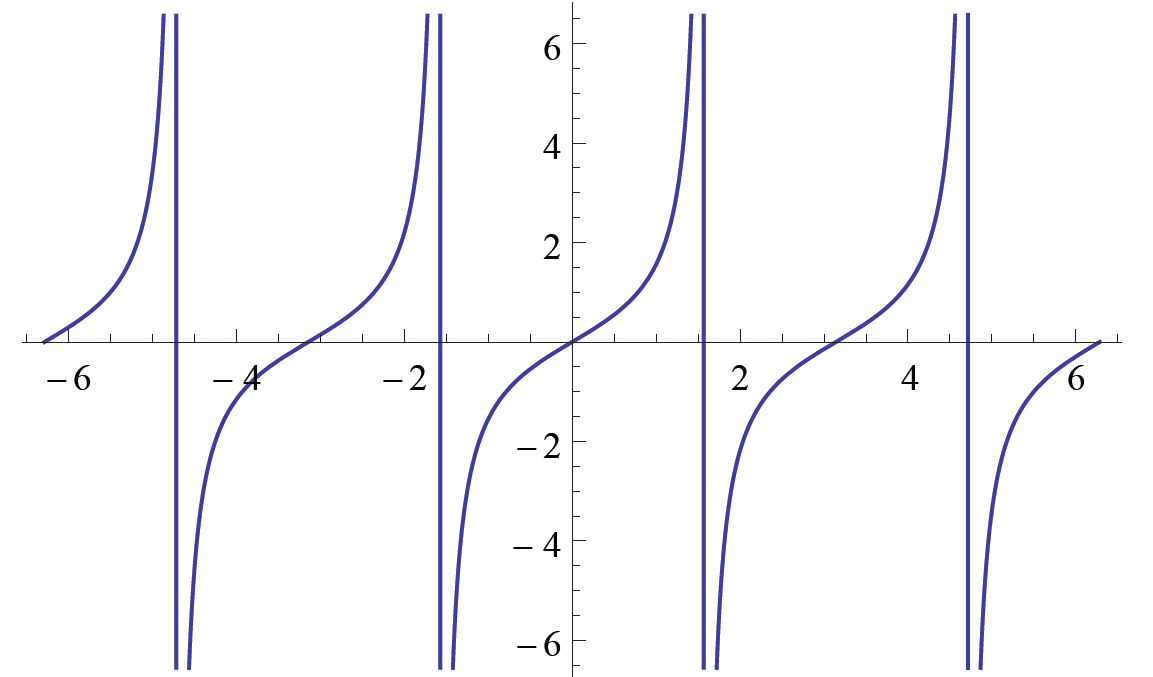
\includegraphics[width=5.5cm]{images/tan.png}
\end{multicols}
\section{Matrizen}
\subsection{Gaussverfahren}
Durch Addition und Subtraktion einzelner Zeilen (auch von Vielfachen einer
Zeile) werden einzelne Stellen auf Null gebracht.\\
\vspace{1.0pt}
$\begin{bmatrix}
a_{11} & a_{12}& \ldots & a_{1n}\\
a_{21}& &\ldots & \\
\ldots \\
a_{n1} & & \ldots & a_{nn}    			
\end{bmatrix}=
\begin{bmatrix}
a_{11} & a_{12}& \ldots & a_{1n}\\
k a_{21}-n a_{11}& ka_{22}-n a_{12}&\ldots & k a_{2n} - n a_{1n}\\
\ldots \\
a_{n1} & & \ldots & a_{nn}    			
\end{bmatrix}$ \\
\vspace{1.0pt}
Die n * erste Zeile wurde von der k * zweiten Zeile abgezogen ($a_{2.}= 
k a_{2.}- n a_{1.}$)

\subsection{Determinante}
\begin{minipage}[t]{6cm}
	\textbf{2x2 Matrix}    
	\[ \det \begin{bmatrix}
	a & b \\
	c & d
	\end{bmatrix} = ad - bc \]
\end{minipage}
\begin{minipage}[t]{12cm}
	\textbf{3x3 Matrix}
	\[\begin{bmatrix}
	a & b & c \\
	d & e & f \\
	g & h & i 
	\end{bmatrix} = aei + bfg + cdh - ceg - afh - bdi \]
\end{minipage}

\subsubsection{Grössere Matrizen}
$$A\epsilon M_n: \det A =    
\begin{vmatrix}
a_{11} & a_{12}& \ldots & a_{1n}\\
a_{21}& &\ldots & \\
\ldots \\
a_{n1} & & \ldots & a_{nn}    			
\end{vmatrix}=
(-1)^{1+1}a_{11}D_{11} + (-1)^{1+2}a_{12}D_{12}+ \ldots +
(-1)^{1+n}a_{1n}D_{1n}$$
\\
\textbf{Unterdeterminante}
$$D_{11}=
\begin{vmatrix}
a_{22} & \ldots & a_{2n}\\
\ldots\\
a_{n2}& \ldots & a_{nn}
\end{vmatrix} 	\\
\qquad
D_{12}=
\begin{vmatrix}
a_{21} & a_{23}& \ldots & a_{2n}\\
\ldots\\
a_{n1}& a_{n3}&\ldots & a_{nn}
\end{vmatrix}$$\\
$D_{ij}$ die (n-1)$ \times $(n-1)-Untermatrix von D ist, die durch Streichen der
i-ten Zeile und j-ten Spalte entsteht.\\
Diese Methode ist zu empfehlen, wenn die Matrix in einer Zeile oder Spalte
bis auf eine Stelle nur Nullen aufweisst.
Dies lässt sich meist mit dem Gausverfahren bewerkstelligen.

\subsection{Inverse Matrix}
Existiert nur wenn Matrix regulär: $\det A \neq 0$\\
\begin{minipage}{7cm}
	\textbf{2x2 Matrix:}    
	$$ A^{-1} = \begin{bmatrix} a & b \\ c & d \\ \end{bmatrix}^{-1} = \frac{1}{ad
		- bc} \begin{bmatrix} d & -b \\ -c & a \\ \end{bmatrix} $$
\end{minipage}
\begin{minipage}{11cm}
	\textbf{3x3 Matrix:}
	$$  A^{-1} = \begin{bmatrix} a & b & c\\ d & e & f \\ g & h & i \\ \end{bmatrix}^{-1} =
	\frac{1}{\det(A)} \begin{bmatrix} ei - fh & ch - bi & bf - ce \\ fg - di & ai
	- cg & cd - af \\ dh - eg & bg - ah & ae - bd \end{bmatrix} $$
\end{minipage}\\

\begin{multicols}{2}
	\subsection{Transponierte Matrix}
	Transponierte Matrix:  $A^T=[a_{ik}^T]=[a_{ki}]$ \\
	vertauschen der Zeilen mit Spalten
	
	\subsection{Einheitsmatrix}
	Einheitsmatrix: $I=E= 
	\begin{bmatrix} 
	1&0 & 0\\
	0&1&0\\
	0&0&1                               
	\end{bmatrix}$	
\end{multicols}

\subsubsection{Grössere Matrizen}
Alle Elemete elementweise invertieren - Kehrwert. $\quad \Rightarrow \quad $\textit{Gilt nur wenn alle Elemente auf der Hauptdiagonale $\neq 0$ sind.}\\

$A^{-1}= \begin{bmatrix}
a_{11} & a_{12}& \ldots & a_{1n}\\
a_{21}& &\ldots & \\
\ldots \\
a_{n1} & & \ldots & a_{nn}    			
\end{bmatrix}^{-1}$

\begin{enumerate}
	\item $A^T$ bestimmen (Zeilen und Spalten vertauschen)
	$ \; A^{T}= \begin{bmatrix}
	a_{11} & a_{21}& \ldots & a_{n1}\\
	a_{12}& &\ldots & \\
	\ldots \\
	a_{1n} & & \ldots & a_{nn}    			
	\end{bmatrix}$	
	\item Bei $A^T$ jedes Element durch Unterdeterminante ersetzen
	$\;A^*=	\begin{bmatrix}
	(-1)^{1+1}D_{11} &  \ldots	& (-1)^{1+n} D_{1n}\\
	\ldots\\
	(-1)^{n+1} D_{n1}& \ldots  & (-1)^{n+n} D_{nn}
	\end{bmatrix}$
	\item $A^{-1} = \frac{A^*}{\det A}$ 
\end{enumerate}


	\subsection{Diagonalisierung}
	\begin{enumerate}
		\item Eigenwerte $\lambda$ ausrechnen: $\det (A - I_n \lambda)=0$
		\item Eigenvektoren $\vec{v}$ bilden: $(A- \lambda I_n)\vec{v}=0$
		\item Transformationsmatrix: $T= [\vec{v_1} \ldots \vec{v_n}]$
		\item $T^{-1}$ berechnen (Achtung ist A symmetrisch, dh. $A^T=A$ und
		oder alle EV senktrecht zueinander, dann $T^{-1}=T^T$)
		\item $D=\begin{bmatrix}
		\lambda_1 &0 &0\\
		0& \lambda_2 &0\\
		0& 0& \lambda_3
		\end{bmatrix} = A_{diag} = T^{-1}AT$
	\end{enumerate}
	
	\subsection{Eigenwerte}
	Die Eigenwerte $\lambda$ erhält man folgendermassen ($I$ ist die Einheitsmatrix):
	\[ |\lambda I - A| = 0 \qquad \text{nach } \lambda \text{ auflösen} \]

\section{Wahrscheinlichkeit}

\clearpage
\pagebreak
\section{Differentialrechnung}
\subsection{Differentation von Funktionen einer Variablen}
Der Differentialquotient oder Ableitung einer Funktion beschriebt die Steigung einer Tangente an die Funktion.\\
\begin{equation*}
f'(x)=\lim\limits_{\triangle x \to 0}\frac{f(x + \triangle x)-f(x)}{\triangle x}
\end{equation*}
Die Ableitung einer Funktion $y=f(x)$ ist eine Funktion von x welche mit den Symbolen: $y'$, $\dot{y}$, $Dy$ dargestellt wird.\\
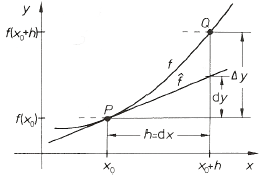
\includegraphics[width=5cm]{images/differential.png}
 
\subsection{Ableitungsregeln}
\renewcommand{\arraystretch}{1.5}
\begin{tabular}{|l|l|}
	\hline \textbf{Konstantenregeln}& $c'=0'$\\
	\hline \textbf{Faktorenregeln}& $(cu)'=c u'$\\
	\hline \textbf{Summenregel}& $(u\pm v)'= u' \pm v'$\\
	\hline \textbf{Produktregel}& $(uv)'=u'v + uv'$\\
	\hline \textbf{Quotientenregel}& $(\frac{u}{v})'= \frac{u'v-uv'}{u^{2}}$\\
	\hline \textbf{Kettenregel}& $y=u(v(x)) ; y'=\frac{du}{dv} \frac{dv}{dx}$\\
	\hline \textbf{Potenzregel} & $(u^{a})'=au^{a-1}$\\
								& $(\frac{1}{u})'= \frac{u'}{u^2}$\\
	\hline	\textbf{Wurzelregel} & $f(x)=\sqrt{x} ; f'(x)=\frac{1}{2\sqrt{x}}$\\
	\hline	\textbf{Logarithmusregel} & $\ln{u}'=\frac{u'}{u}$\\ 
	\hline	\textbf{Differentation der Umkehrfunktion} & $(f^{-1})'(y)=\frac{1}{f'(x)} $\\
	\hline 
\end{tabular}
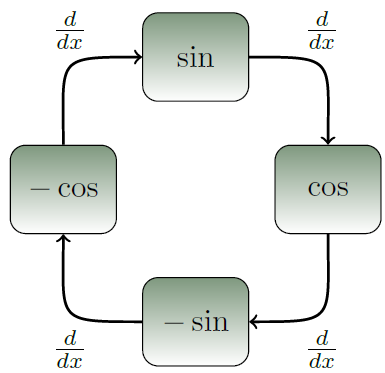
\includegraphics[width=5cm]{images/sin_cos.png}
\newpage
\subsection{Ableitungen elementarer Funktionen}
\renewcommand{\arraystretch}{2.2}
\begin{tabular}{|l|l||l|l|}
	\hline
	\textbf{Funktion} & \textbf{Ableitung} & \textbf{Funktion} &
	\textbf{Ableitung}\\\hline
	\hline $C$ (Konstante) & 0 & $\sec x$ & $\dfrac{\sin x}{\cos^2 x}$ \\
	\hline $x$ & 1 & $\sec^{-1} x$ & $\dfrac{-\cos x}{\sin^2 x}$\\
	\hline $x^n$ ($n\in\mathbb{R}$) & $nx^{n-1}$ & $\arcsin x \quad (|x| < 1)$ &
	 $\dfrac{1}{\sqrt{1-x^2}}$\\
	\hline $\dfrac{1}{x}$ & $-\dfrac{1}{x^2}$ & $\arccos x \quad (|x| < 1)$ &
	$-\dfrac{1}{\sqrt{1-x^2}}$\\
	\hline $\dfrac{1}{x^n}$ & $-\dfrac{n}{x^{n+1}}$ & $\arctan x$ & $\dfrac{1}{1+x^2}$\\
	\hline $\sqrt{x}$ & $\dfrac{1}{2\sqrt{x}}$ & $\arccot{x} $ & $-\dfrac{1}{1+x^2}$\\
	\hline $\sqrt[n]{x}\quad (n\in\mathbb{R}, n \neq 0, x > 0)$ &
	$\dfrac{1}{n\sqrt[n]{x^{n-1}}}$ & $\arcsec x$ & $\dfrac{1}{x\sqrt{x^2-1}}$\\
	\hline $\mathrm{e}^x$ & $\mathrm{e}^x$ & $\arcossec x$ & $-\dfrac{1}{x\sqrt{x^2-1}}$\\
	\hline $\mathrm{e}^{bx}\quad (b\in\mathbb{R})$ & $b\mathrm{e}^{bx}$ & $\sinh x$ &
	$\cosh x$\\
	\hline $a^x\quad (a > 0)$ & $a^x\ln a$ & $\cosh x$ & $\sinh x$\\
	\hline $a^{bx}\quad (b\in\mathbb{R}, a > 0)$ & $ba^{bx}\ln a$ & $\tanh x$ &
	$\dfrac{1}{\cosh^2 x}$\\
	\hline $\ln x$ & $\dfrac{1}{x}$ & $\coth x \quad(x \neq 0)$ & $-\dfrac{1}{\sinh^2 x}$\\
	\hline $\log_a{x} \quad (a > 0, a \neq 1, x > 0)$ &
	$\dfrac{1}{x}\log_a{\mathrm{e}}=\dfrac{1}{x\ln a}$ & $\arsinh x$ &
	$\dfrac{1}{\sqrt{1+x^2}}$\\
	\hline $\lg x \quad (x > 0)$ & $\dfrac{1}{x}\lg \mathrm{e}\approx \dfrac{0.4343}{x}$
	& $\arcosh x \quad (x > 1)$ & $\dfrac{1}{\sqrt{x^2-1}}$\\
	\hline $\sin x$ & $\cos x$ & $\artanh x \quad (|x| < 1)$ & $\dfrac{1}{1-x^2}$\\
	\hline $\cos x$ & $-\sin x$ & $\arcoth x \quad (|x| > 1)$ & $-\dfrac{1}{x^2-1}$\\
	\hline $\tan x \quad (x\neq(2k+1)\dfrac{\pi}{2}, k\in\mathbb{Z})$ & $\dfrac{1}{\cos^2
		x}=\sec^2 x$ & $[f(x)]^n \quad (n\in\mathbb{R})$ & $n[f(x)]^{n-1}f'(x)$\\
	\hline $\cot x \quad (x\neq k\pi, k\in\mathbb{Z})$ & $\dfrac{-1}{\sin^2 x}=-cosec^2x$ & $\ln f(x) \quad (f(x)> 0)$ & $\dfrac{f'(x)}{f(x)}$\\
	\hline
\end{tabular}
\newpage
\section{Integralrechung}
Die Integralrechnung ist die Umkehrung der Differentialrechnung. Bei der Differentialrechnung wird zu einer gegebenen Funktion $f(x)$ die Ableitung $f'(x)$ bestimmt. Bei der Integralrechung wird zu eine Ableitung $f'(x)$ eine Funktion $f(x)$ gesucht welche mit der Ableitung übereinstimmt. 
\begin{equation*}
	F'(x)=\frac{dF}{dx}=f(x)
\end{equation*}
\begin{tabular}{|c|c|}
	\hline \textbf{Bestimmtes Integral} & \textbf{Unbestimmtes Integral}\\
	\hline $\int_{a}^{b}{f(x)dx}$ & $\int{f(x)dx}=F(x)+C$\\
	\hline \tabbild[width=4cm]{images/best_integral.png}& \tabbild[width=4cm]{images/unb_integral.png}\\
	\hline
\end{tabular}

\subsection{Integrationsregeln}
\begin{tabular}{|l|l|l|}
	\hline	\textbf{Integrationskonstane} & $\int{f(x)dx}=F(x)+C$&\\
	\hline	\textbf{Faktorregel}& $\int{af(x)dx}=a \int{f(x)dx}$&\\
	\hline	\textbf{Summenregel}& $\int{[u(x) \pm v(x)]dx}=\int{u(x)dx} \pm \int{v(x)dx}$&\\
	\hline \textbf{Potenzregel}& $\int {f'(x)\cdot f(x)^{a}}=\frac{f(x)^{a+1}}{a+1}+C$& $\int {\sin^3{(x)} \cdot \cos(x)}=\frac{\sin^4{(x)}}{4}+C$\\
	\hline \textbf{Logarithmusregel} & $\int{\frac{f'(x)}{f(x)}dx}= \ln{(x)}+C$&$\int{\frac{x^2}{1+x^3}}=\ln(1+x^3)+C$ \\
	\hline \textbf{Linearität} &$\int{f(ax \pm b)dx}=\frac{1}{a} \int{f(x)dx} \pm \int{b dx}$&\\
	\hline \textbf{Partielle Integration} &$\int{u(x)v'(x)dx}=u(x)v(x)- \int{u'(x)v(x)dx}$ &$\int{ \underbrace{x^2}_{v'} \cdot \underbrace{\ln{x}}_{u}}=\frac{x^3}{3} \cdot \ln{x} - \int{\frac{x^3}{3} \cdot \frac{1}{x}}$\\
			\textbf{(Produktregel)} & &\\
	\hline	\textbf{Substitution} &$\int_{a}^{b}{f(x)dx}=\int_{g(a)}^{g(b)}{f(g(t))\cdot g'(t)dt}$  &$\int{(x^2+2)^3 \cdot 2xdx}\;\;//\;u=x^2+2$\\
	& &$\int{u^3 \cdot 2xdx}\;\;//\;du=2xdx$\\
	& &$\int{u^3 \cdot du}=\frac{u^4}{4}=\frac{(x^2+2)^4}{4}$\\
	\hline
\end{tabular}

\subsection{Wichtige Integrale}
\renewcommand{\arraystretch}{2}
\begin{tabular}{|l|l|}
	\hline
	$\int \sin(x)dx=-\cos(x)$ & $\int \sin(a+bx)dx=-\frac1b \cos(a+bx)$\\
	\hline
	$\int \sin^2(x)dx=-\frac14 \sin(2x)+\frac x2$ 
	& $\int
	e^{ax+c}\sin(bx+d)dx=\frac{e^{ax+c}}{a^2+b^2}(a\sin(bx+d)-b\cos(bx+d))$\\
	\hline
	$\int \cos(x)dx=\sin(x)$ & $\int \cos(a+bx)dx=\frac1b \sin(a+bx)$\\
	\hline
	$\int \cos^2(x)dx=\frac14 \sin(2x)+\frac x2$ 
	& $\int
	e^{ax+c}\cos(bx+d)dx=\frac{e^{ax+c}}{a^2+b^2}(a\cos(bx+d)+b\sin(bx+d))$\\
	\hline
	$\int e^x dx=e^x$ & $\int e^{ax}dx=\frac1a e^{ax}$\\
	\hline
	$\int xe^{ax}dx=\frac{1}{a^2} e^{ax}(ax-1)$ & $\int x^2 e^{ax} dx =
	e^{ax}\left( \frac{x^2}{a} - \frac{2x}{a^2} + \frac{2}{a^3}\right)$ \\
	\hline
	$\int x^n e^{ax} dx = \frac{1}{a} x^n e^{ax} - \frac{n}{a} \int x^{n-1}
	e^{ax} dx$ & \\
	\hline
\end{tabular}
\newpage
\section{Fourierreihen}
Mithilfe der Fourierreihe kann ein beliebiges periodisches Signal in seine Grundschwingungen (Harmonische) aufgeteilt werden.\\
%\renewcommand{\arraystretch}{2}
\begin{tabular}{|l|l|}
	\hline \textbf{Fourierreihe} &${f(t) = \frac{a_0}{2} + \sum\limits_{k=1}^{\infty} \left[a_k \cos(k
		\omega t) + b_k \sin(k \omega t)\right]} \rightarrow FR[f(t)] \; \omega=\frac{2 \pi}{T}=2 \pi$\\
	\hline \textbf{Berechnung Reell} & $a_0 = \frac{2}{T}\int\limits_0^{T}
	f(t)dt, \quad a_k = \frac{2}{T}\int\limits_0^{T} f(t)\cos(k \omega_1 t) dt, \quad b_k =
	\frac{2}{T}\int\limits_0^{T} f(t)\sin(k \omega_1 t) dt$\\
	\hline \textbf{Berechnung komplex} & $c_k=\frac{1}{T}\int_0^T{f(t)}\cdot
		e^{-jk\omega t}, \quad f(t) = \sum\limits_{k = -\infty}^{\infty} c_k \cdot e^{j k \omega t dt}$\\
	\hline
\end{tabular}

\subsection{Symmetrie}
\begin{tabular}{|l|l|l|l|}
	\hline
	\textbf{gerade Funktion} & \textbf{ungerade Funktion} &
	\textbf{Halbperiode 1} & \textbf{Halbperiode 2}\\
	\hline
	\tabbild[width=3cm]{images/gerade_funktion.png}&
	\tabbild[width=3cm]{images/ungerade_funktion.png}&   
	\tabbild[width=3cm]{images/halbperiode_1.png}&   
	\tabbild[width=3cm]{images/halbperiode_2.png}\\
	\hline $f(-t)=f(t)$ & $f(-t)=-f(t)$ & $f(t)=f(t+\pi)$ & $f(t)=-f(t+\pi)$\\
	$b_k=0$ & $a_k=0$ & $a_{2k+1}=0$ & $a_{2k}=0$\\
	$a_k = \frac{4}{T} \int\limits_0^{\frac{T}{2}} f(t) \cdot \cos(k \omega_1
	t) dt$ &
	$b_k =  \frac{4}{T} \int\limits_0^{\frac{T}{2}} f(t) \cdot
	\sin(k \omega_1 t) dt$ &
	$b_{2k+1}=0$ & $b_{2k}=0$\\
	\hline $\Im(c_n)=0$ &$\Re(c_n)$ & &\\ 
	\hline
\end{tabular}

\subsection{Wichtige Fouriereihen}
\begin{tabular}{|l|l|l|}
	\hline \textbf{Dreieckfunktion} & \textbf{Rechteckfunktion}& \textbf{Impulsfunktion}\\
	\hline \tabbild[width=4cm]{images/dreiecksig.png} &\tabbild[width=4cm]{images/rechteck.png}&\tabbild[width=4cm]{images/impuls.png}\\
	\hline $a_0=A$& $a_0=0$& $a_0=\frac{2At_1}{T}$\\
	\hline $a_k=-\frac{4A}{\pi^{2}k^{2}}$&$a_k=0$&$a_k=\frac{A}{\pi k}(\sin(\frac{2 \pi t_1}{T}k))$\\
	\hline $b_k=0$&$b_k=\frac{4A}{\pi k}$&$b_k=-\frac{A}{\pi k}(1-\cos(\frac{2 \pi t_1}{T}k))$\\
	\hline
\end{tabular}
\clearpage
\pagebreak
\section{Fouriertransformation}
Mithilfe der Fouriertransformierten kann ein endliches nicht periodisches Signal analysiert werden. Dazu wechselt man vom Zeitbereich in den Frequenzbereich.\\
\begin{tabular}{|l|l|}
	\hline \textbf{Fourierintegral} & $F(j\omega) = \int\limits_{-\infty}^{\infty} f(t)e^{-j\omega t}dt$\\
	\hline \textbf{Rücktransformierte} &$\frac{1}{2\pi}\int\limits_{-\infty}^{\infty}
	F(j\omega)e^{j\omega t}d\omega$\\
	\hline
\end{tabular}

\subsection{Eigenschaften der Fouriertransformierten}
\begin{tabular}{|l|l|}
	\hline
	Linearität & 
	$\alpha\cdot f(t) + \beta\cdot g(t) \;\laplace\;\alpha\cdot F(j\omega) +
	\beta\cdot G(j\omega)$\\
	\hline
	Zeitumkehrung (Spiegelung an der Y-Achse)&
	$f(-t) \;\laplace\; F(-j\omega) = F^*(jw)$ \\
	\hline        	
	Streckung im Zeitbereich &
	$f(\alpha t) \;\laplace\; \frac{1}{|\alpha|}F \left (j\frac{\omega}{\alpha} \right)
	\quad\alpha \in\mathbb{R}\setminus \{0\}$\\
	\hline
	Verschiebung im	Zeitbereich &
	$f(t\pm t_0) \;\laplace\; F(j\omega)e^{\pm j\omega t_0}$\\
	\hline
	Verschiebung im Frequenzbereich &
	$f(t)e^{\pm j\omega_0 t} \;\laplace\; F(j(\omega\mp\omega_0))$\\
	\hline
	Ableitung im Zeitbereich &
	$\frac{\partial^n f(t)}{\partial t^n} \;\laplace\; (j\omega)^n F(j\omega)$\\
	\hline
	Integration im Zeitbereich &
	$\int\limits_{-\infty}^{t}f(\tau)d\tau \;\laplace\;
	\frac{F(j\omega)}{j\omega}+F(0)\pi\delta(\omega)$\\
	\hline				
	Ableitung im Frequenzbereich &
	$t^n f(t) \;\laplace\; j^n \frac{\partial F(j\omega)}{\partial \omega^n}$\\
	\hline		
	Faltung im Zeitbereich &
	$f(t) \ast g(t) = \int\limits_{-\infty}^{\infty} f(\tau)g(t-\tau)d\tau \;\laplace\;
	F(j\omega) \cdot G(j\omega)$\\
	\hline
	Faltung im Frequenzbereich &
	$f(t) \cdot g(t) \;\laplace\; \frac{1}{2\pi}F(j\omega) \ast G(j\omega)$\\
	\hline
	Vertauschungssatz (Dualität) &
	$f(t) \;\laplace\; F(j\omega)\nonumber$ \\
	& $F(t) \;\Laplace\; 2\pi \cdot f(-j\omega)$\\
	\hline
	Modulation &
	$\cos(\alpha t) \cdot f(t)  \;\laplace\;  \frac{1}{2}\cdot
	\left[F(j(\omega-\alpha)) + F(j(\omega+\alpha))\right ]$\\
	& $\sin(\alpha t) \cdot f(t) \;\laplace\; \frac{1}{2j}\cdot \left[
	F(j(\omega-\alpha)) - F(j(\omega+\alpha))\right ]$\\
	\hline
	Parseval's Theorem &
	$\int\limits_{-\infty}^{\infty}f(t)g^{\ast}(t)dt = \frac{1}{2\pi}
	\int\limits_{-\infty}^{\infty}F(j\omega)G^{\ast}(j\omega)d\omega$\\
	\hline
	Bessel's Theorem &
	$\int\limits_{-\infty}^{\infty}|f(t)|^2 dt = \frac{1}{2\pi}
	\int\limits_{-\infty}^{\infty}|F(j\omega)|^2 d\omega$\\
	\hline 			
	Anfangswerte &
	$f(0)=\frac{1}{2\pi}\int\limits_{-\infty}^{\infty}F(j\omega)d\omega
	\hspace*{1cm} F(0)=\int\limits_{-\infty}^{\infty}f(t)dt$\\
	\hline
	$\infty$ lange Folge von $\delta$-Impulsen &
	$\sum_{n=-\infty}^{\infty} \delta(t-n\cdot t_0) \;\laplace\;
	\sum_{n=-\infty}^{\infty} \frac{2\pi}{t_0}\delta(\omega-n\cdot
	\frac{2\pi}{t_0})$\\
	\hline
\end{tabular}

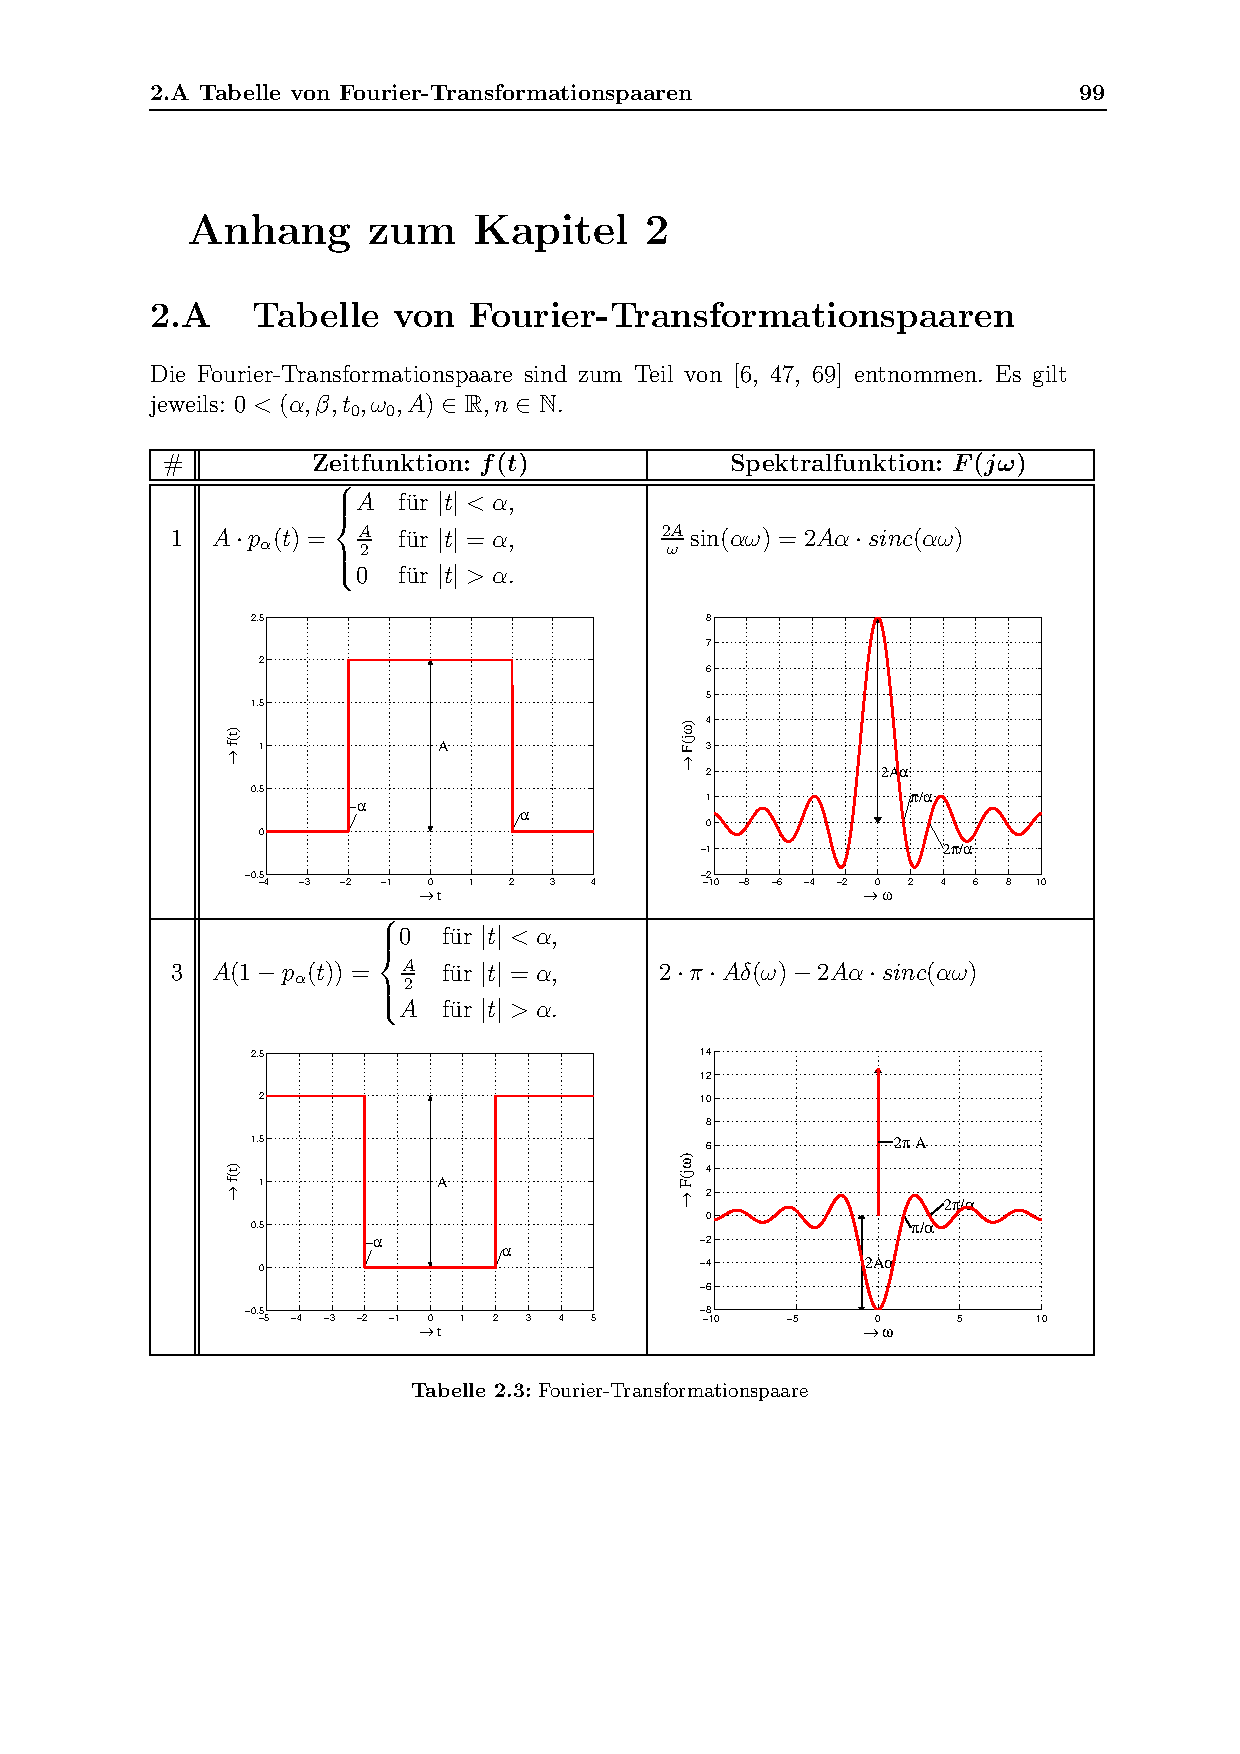
\includepdf[pages={1-7}]{sections/Tabellen.pdf}
\section{Laplacetransformation}
Mittels der Laplacetransforamtion können kausale Signale analysiert werden. Sollte das Signal nicht kausal sein wird es mit der Einschaltfunktion multipliziert.\\
\begin{tabular}{c}
	$F(s)=\int\limits_0^\infty f(t)e^{-st}dt \qquad s=\sigma+j\omega$\\
	$Originalbereich \;\laplace\; Bildbereich$\\
\end{tabular}

\subsection{Eigenschaften der Laplacetransformation}
\begin{tabular}{|l|l|}
	\hline
	Linearität & 
	$\alpha\cdot f(t) + \beta\cdot g(t) \;\laplace\; \alpha\cdot F(s) + \beta\cdot
	G(s)$ \\
	\hline
	Zeitskalierung &
	$f(\alpha t) \;\laplace\; \frac{1}{\alpha}F \left (\frac{s}{\alpha} \right ) \quad 0
	<\alpha \in\mathbb{R}$ \\
	\hline
	Faltung im Zeitbereich &
	$f(t) \ast g(t) = \int\limits_{0}^{\infty} f(\tau)g(t-\tau)d\tau \;\laplace\; F(s)
	\cdot G(s)$\\
	\hline
	Faltung im Frequenzbereich &
	$f(t) \cdot g(t) \;\laplace\; \frac{1}{2\pi j}\int\limits_{c-j\infty}^{c+j\infty}
	F(\xi) G(s-\xi)d\xi$ \\
	\hline
	Ableitung im Zeitbereich &
	$\frac{\partial f(t)}{\partial t} \;\laplace\; sF(s)
	-f(0+)$ \\
	\hline
	Ableitungen im Zeitbereich &
	$\frac{\partial^n f(t)}{\partial t^n} \;\laplace\; s^nF(s)
	-s^{n-1}f(0+)-s^{n-2}\frac{\partial f(0+)}{\partial t}-\ldots
	-s^0\frac{\partial^{n-1} f(0+)}{\partial t^{n-1}}$ \\
	\hline
	Multiplikation mit $t$ &
	$t\cdot f(t)  \;\laplace\; \frac{-\partial F(s)}{\partial s}$ \\
	\hline
	Ableitung im Frequenzbereich &
	$(-t)^n f(t) \;\laplace\;  \frac{\partial^n F(s)}{\partial s^n}$ \\
	\hline
	Verschiebung im Zeitbereich &
	$f(t\pm t_0) \;\laplace\; F(s)e^{\pm t_0 s}$ \\
	\hline
	Verschiebung im Frequenzbereich &
	$f(t)e^{\mp\alpha t} \;\laplace\; F(s\pm\alpha)$ \\
	\hline
	Integration &
	$\int\limits_0^t f(\tau)d\tau \;\laplace\; \frac{F(s)}{s}$ \\
	\hline
	Anfangswert &
	$\lim_{t\rightarrow 0} f(t) = \lim_{s\rightarrow \infty} sF(s),\text{~wenn
	}  \lim_{t\rightarrow 0} f(t)\text{~existiert}.$ \\
	\hline
	Endwert &
	$\lim_{t\rightarrow \infty} f(t) = \lim_{s\rightarrow 0} sF(s),\text{~wenn
	}  \lim_{t\rightarrow \infty} f(t)\text{~existiert}.$ \\
	\hline
\end{tabular}
\newpage
\subsection{Rücktransformation}
\subsubsection{Vorgehen}
\begin{minipage}{12cm}
	\begin{enumerate}
		\item Benutzung einer Tabelle zugehöriger Original-, und Bildfunktionen (Korrespondenzen)
		\item Umformen (Kürzen, Erweitern, etc.) um auf Korrespondenz zu schliessen
		\item Mittels Partialbruchzerlegung auf Korrespondenz schliessen
	\end{enumerate}
\end{minipage}
\begin{minipage}{7cm}
	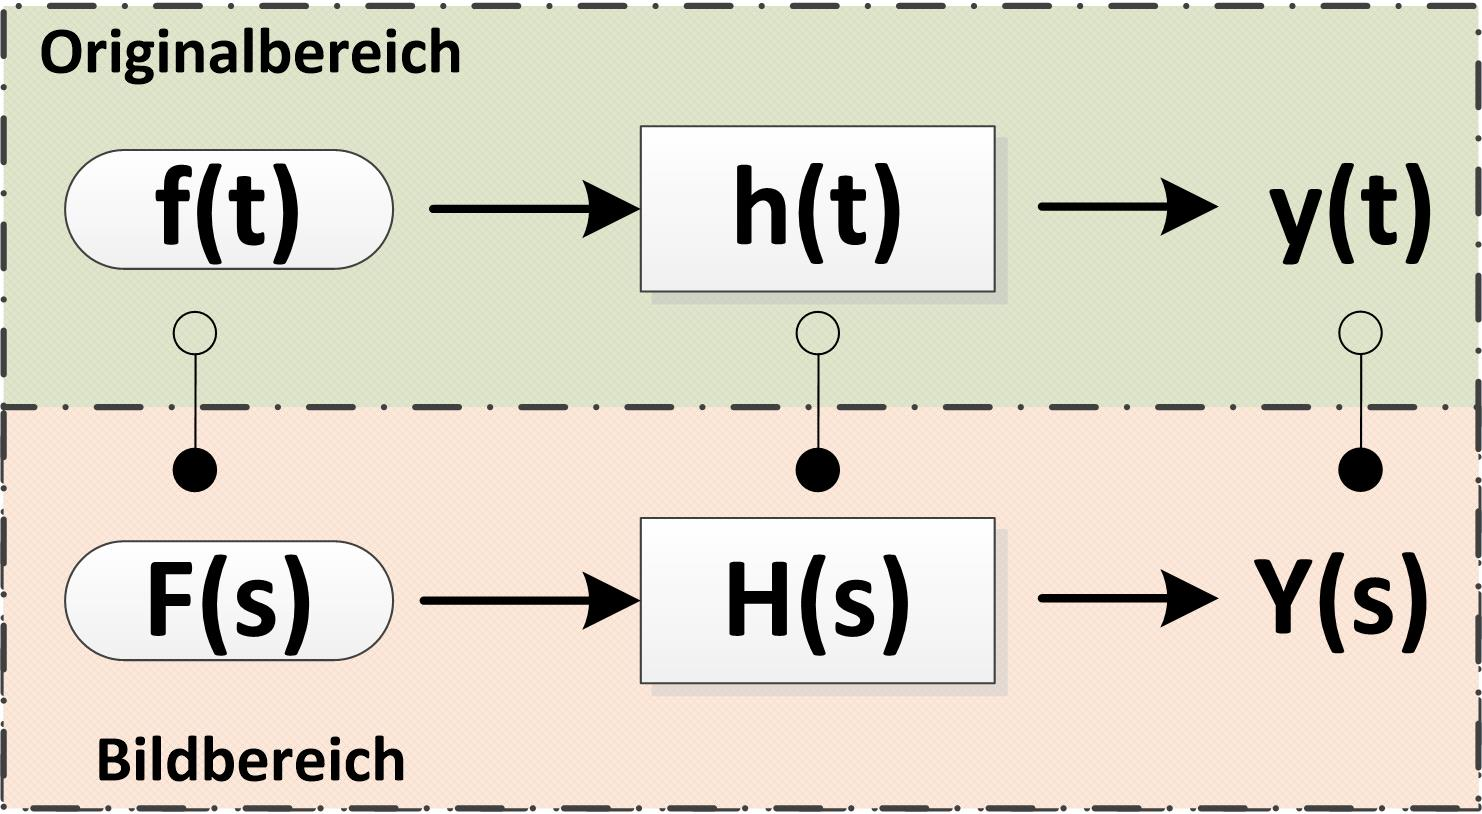
\includegraphics[width=7cm]{images/IntTra.jpg}
\end{minipage}

\subsubsection{Laplacetabelle}
\begin{multicols}{2}
	\begin{center}
		\begin{tabular}{|lcc|}
			\hline
			$\sigma \left( t \right)$ & $\; \laplace \;$ & $\frac{1}{s}$ \\
			$\sigma \left( t \right) \cdot t$ & $\; \laplace \;$ & $\frac{1}{s^2}$\\
			$\sigma \left( t \right) \cdot t^2$ & $\; \laplace \;$ & $\frac{2}{s^3}$\\
			$\sigma \left( t \right) \cdot t^n$ & $\; \laplace \;$ & $\frac{n!}{s^{n+1}}$\\
			$\sigma \left( t \right) \cdot e^{\alpha t}$ & $\; \laplace \;$ &
			$\frac{1}{s-\alpha}$\\
			$\sigma \left( t \right) \cdot t \cdot e^{\alpha t}$ & $\; \laplace \;$ &
			$\frac{1}{( s - \alpha )^2}$\\
			\hline
		\end{tabular}
	\end{center}
	\columnbreak
	\begin{center}
		\begin{tabular}{|lcc|}
			\hline
			$\sigma \left( t \right)\cdot t^2 \cdot e^{\alpha t}$ &
			$\; \laplace \;$ & $\frac{2}{{( s - \alpha )}^3}$\\
			$\sigma \left( t \right)\cdot t^n \cdot e^{ \alpha t}$ &
			$\; \laplace \;$ & $\frac{n!}{(s-\alpha)^{n+1}}$\\
			$\sigma \left( t \right) \cdot \sin \left(\omega t \right)$ & $\; \laplace \;$ &
			$\frac{\omega}{s^2 + {\omega^2}}$\\
			$\sigma \left( t \right) \cdot \cos \left( \omega t \right)$ & $\; \laplace \;$ &
			$\frac{s}{ s^2 + \omega^2}$\\
			$\delta \left( t \right)$ & $\; \laplace \;$ & $1\left( s \right)$ \\
			$\delta \left( t - \alpha \right)$ & $\; \laplace \;$ & $e^{- \alpha s}$\\
			\hline
		\end{tabular}
	\end{center}
\end{multicols}

\subsection{Lösen von Differentialgleichungen mit Laplace}
\begin{minipage}{11.5cm}
	\begin{tabular}{| l | l |}
		\hline
		Übertragungsfunktion & $G(s) = \frac{1}{p(s)} \quad g(t) \; \laplace \; G(s)$\\
		\hline Charakteristisches Polynom & $p(s)$\\
		\hline
		Frequenzgang & $G(j\omega) = H(\omega)$ \\
		\hline
		Impulsantwort & $y_{\delta}(t) = g(t) = y_{\sigma}'(t) \; \laplace \; G(s) = \frac{1}{p(s)}=Y_{\delta}(s)$\\
		\hline
		Sprungwantwort & $y_{\sigma}(t)=\int\limits_0^t g(u) du \; \laplace \; \frac{G(s)}{s} = \frac{1}{s \cdot p(s)} = Y_{\sigma}(s)$\\
		\hline
		Eigenschwingung & $\frac{h(s)}{p(s)}$ \\
		\hline
		äussere Erregung & $\frac{F(s)}{p(s)}$ \\
		\hline
		stationärer Zustand & = ungedämpfte Eigenschwingung\\
		\hline
	\end{tabular}
\end{minipage}
\newpage
\subsubsection{Lineare DGL mit Anfangswerten}
Gegeben sei eine Differentialgleichung mit Anfangsbedingungen.Sind keine Anfangsbedingungen vorhanden können die daraus entstehenden Terme vernachlässigt werden.\\
\vspace{2pt}
\begin{tabular}{l l}
	DGL & $a_n y^{n}(t)+a_n-1 y^{n-1}+...a_1 y'(t)+a_0 y(t)=f(t)$\\
	Endterm & $a_0\cdot[Y(s)]+a_1 \cdot [sY(s)-f(0)]+a_n-1y^n-1 \cdot [s^nY(s)-s^{n-1} \cdot f(0)-s^{n-2}f'(0)...-f^{n-1}(0)]=F(s)$\\
\end{tabular}

\begin{minipage}{15cm}
	$y(t) \; \laplace \;  Y(s)$\\
	$y'(t) \; \laplace \; sY(s) - f(0)$\\
	$y''(t) \; \laplace \; s^2Y(s)-s\cdot f(0) - f'(0)$\\
	$y'''(t) \; \laplace \; s^3Y(s)-s^2\cdot f(0)-s \cdot f'(0) - f''(0)$\\
	$y^n(t) \; \laplace \; s^nY(s)-s^{n-1}\cdot f(0)-s^{n-2} \cdot f'(0) ...- f^{n-1}(0)$\\
	$y^{(n)} \; \laplace \; 
	\underbrace{s^nY(s)}_{Y(s) \cdot p(s)}
	\underbrace{-s^{n-1}y_0 - \dots - y^{(n-1)}}_{h(s)}$\\
\end{minipage}
\newpage
\includepdf[pages={8-9}]{sections/Tabellen.pdf}
\input{sections/logischeOperationen}
\input{sections/nassiShneidermann}
\section{Signale}
\subsection{Harmonische Schwingungen}
Als harmonische Schwingung bezeichnet man eine sinusförmige Schwingung. 
\begin{equation*}
x(t) \underbrace{A}_{Amplitude} \cdot \sin(\underbrace{\omega}_{Kreisfrequenz}t +\underbrace{\phi}_{Phasenverschiebung})+\underbrace{c}_{DC-Anteil}
\end{equation*}
\begin{tabular}{|l|l|l|}
	\hline
	\textbf{Ordnung n}& \textbf{Frequenz}& \textbf{Name der Komponente}\\
	\hline $0$& $0$& Gleichstromanteil\\
	\hline $1$& $f_0$& Grundwelle / 1.Harmonische\\
	\hline $2$& $2f_0$& 1.Oberwelle / 2.Harmonische\\
	\hline $3$& $3f_0$& 2.Oberwelle/ 3.Harmonische\\
	\hline $n$& $nf_0$& n-1.Oberwelle / n-te .Harmonische\\
	\hline
\end{tabular}
\clearpage
\pagebreak
%TODO Fehler font beheben
\subsection{Logarithmische Darstellungen}
\renewcommand{\arraystretch}{1.2}
\begin{tabular}{ll}
	\parbox{7cm}{
		\scriptsize
		\begin{tabular}{|c|c|c|c|}
			\hline
			\textbf{Lrel. (dB)} & \textbf{Lrel. (NP)} & \textbf{P2/P1} & \textbf{A2/A1} \\ \hline
			$100.000$ & $11.513$ & $10^{10}$ & $10^5$ \\ \hline
			$90.000$ & $10.362$ & $10^9$ & $31622.777$ \\ \hline
			$80.000$ & $9.210$ & $10^8$ & $10^4$ \\ \hline
			$70.000$ & $8.059$ & $10^7$ & $3162.278$ \\ \hline
			$60.000$ & $6.908$ & $10^6$ & $10^3$ \\ \hline
			$50.000$ & $5.756$ & $10^5$ & $316.228$ \\ \hline
			$40.000$ & $4.605$ & $10^4$ & $10^2$ \\ \hline
			$30.000$ & $3.454$ & $10^3$ & $31.623$ \\ \hline
			\textbf{$20.000$} & $2.303$ & \textbf{$10^2$} & \textbf{$10.000$} \\ \hline
			$19.085$ & $2.197$ & $81.000$ & $9.000$ \\ \hline
			$19.000$ & $2.187$ & $79.433$ & $8.913$ \\ \hline
			$18.062$ & $2.079$ & $64.000$ & $8.000$ \\ \hline
			$18.000$ & $2.072$ & $63.096$ & $7.943$ \\ \hline
			$17.000$ & $1.957$ & $50.119$ & $7.079$ \\ \hline
			$16.902$ & $1.946$ & $49.000$ & $7.000$ \\ \hline
			$16.000$ & $1.842$ & $39.811$ & $6.310$ \\ \hline
			$15.563$ & $1.792$ & $36.000$ & $6.000$ \\ \hline
			$15.000$ & $1.727$ & $31.623$ & $5.623$ \\ \hline
			$14.000$ & $1.612$ & $25.119$ & $5.012$ \\ \hline
			\textbf{$13.979$} & $1.609$ & \textbf{$25.000$} & \textbf{$5.000$} \\ \hline
			$13.000$ & $1.497$ & $19.953$ & $4.467$ \\ \hline
			\textbf{$12.041$} & $1.386$ & \textbf{$16.000$} & \textbf{$4.000$} \\ \hline
			\textbf{$12.000$} & $1.382$ & $15.849$ & $3.981$ \\ \hline
			$11.000$ & $1.266$ & $12.589$ & $3.548$ \\ \hline
			\textbf{$10.000$} & $1.151$ & \textbf{$10.000$} & $3.162$ \\ \hline
			$9.542$ & $1.099$ & $9.000$ & $3.000$ \\ \hline
			$9.000$ & $1.036$ & $7.943$ & $2.818$ \\ \hline
			$8.000$ & $0.921$ & $6.310$ & $2.512$ \\ \hline
			$7.000$ & $0.806$ & $5.012$ & $2.239$ \\ \hline
			\textbf{$6.021$} & \textbf{$0.693$} & \textbf{$4.000$} & \textbf{$2.000$} \\ \hline
			$6.000$ & $0.691$ & $3.981$ & $1.995$ \\ \hline
			$5.000$ & $0.576$ & $3.162$ & $1.778$ \\ \hline
			$4.000$ & $0.461$ & $2.512$ & $1.585$ \\ \hline
			\textbf{$3.010$} & \textbf{$0.347$} & \textbf{$2.000$} & \textbf{$1.414$} \\ \hline
			$3.000$ & $0.345$ & $1.995$ & $1.413$ \\ \hline
			$2.000$ & $0.230$ & $1.585$ & $1.259$ \\ \hline
			$1.000$ & $0.115$ & $1.259$ & $1.122$ \\ \hline
			$0.000$ & $0.000$ & $1.000$ & $1.000$ \\ \hline
			-$1.000$ & -$0.115$ & $0.794$ & $0.891$ \\ \hline
			-$2.000$ & -$0.230$ & $0.631$ & $0.794$ \\ \hline
			-$3.000$ & -$0.345$ & $0.501$ & $0.708$ \\ \hline
			-$4.000$ & -$0.461$ & $0.398$ & $0.631$ \\ \hline
			-$5.000$ & -$0.576$ & $0.316$ & $0.562$ \\ \hline
			-$6.000$ & -$0.691$ & $0.251$ & $0.501$ \\ \hline
			-$7.000$ & -$0.806$ & $0.200$ & $0.447$ \\ \hline
			-$8.000$ & -$0.921$ & $0.158$ & $0.398$ \\ \hline
			-$9.000$ & -$1.036$ & $0.126$ & $0.355$ \\ \hline
			-$10.000$ & -$1.151$ & $0.100$ & $0.316$ \\ \hline
			-$15.000$ & -$1.727$ & $0.032$ & $0.178$ \\ \hline
			-$20.000$ & -$2.303$ & $10^{-2}$ & $0.100$ \\ \hline
			-$30.000$ & -$3.454$ & $10^{-3}$ & $0.032$ \\ \hline
			-$40.000$ & -$4.605$ & $10^{-4}$ & $0.010$ \\ \hline
			-$50.000$ & -$5.756$ & $10^{-5}$ & $0.003$ \\ \hline
			-$60.000$ & -$6.908$ & $10^{-6}$ & $0.001$ \\ \hline
			-$70.000$ & -$8.059$ & $10^{-7}$ & $0.000$ \\ \hline
			-$80.000$ & -$9.210$ & $10^{-8}$ & $10^{-4}$ \\ \hline
			-$90.000$ & -$10.362$ & $10^{-9}$ & $3.162 \cdot 10^{-5}$ \\ \hline
			-$100.000$ & -$11.513$ & $10^{-10}$ & $10^{-5}$ \\ \hline
		\end{tabular}
	}
	& \parbox{11.5cm}{
		\normalsize
		Verstärkungsmass L in \textbf{Dezibel} (dB):\\
		$L_P = 10 \cdot \log \left(\frac {P_2} {P_1}\right) \qquad$ Index P: Leistung \\
		$L_A = 20 \cdot \log \left(\frac {A_2} {A_1}\right) \qquad$ Index A: Amplitude \\ 
		
		Dezibel L zu linear: \\
		$P_2 = P_1 \cdot 10^{\frac{L_P}{10}} $ \\
		$A_2 = A_1 \cdot 10^{\frac{L_A}{20}} $ \\
		
		Verstärkungsmass L in \textbf{Neper} (Np):\\
		$L_P = \frac {1}{2} \cdot \ln \left(\frac {P_2} {P_1}\right)$\\
		$L_A = \ln \left(\frac {A_2} {A_1} \right)$ \\
		
		Neper zu linear: \\
		$P_2 = P_1 \cdot e^{2 L_P}$ \\
		$A_2 = A_1 \cdot e^{L_A}$ \\
		
		Die Umrechnung zwischen {\bf dB} und {\bf Np} ist linear: \\
		$1\mbox{~dB} = \frac {\ln(10)} {20} \mbox{~Np} = 0.1151\mbox{~Np}$ \\
		$1\mbox{~Np} = 20 \cdot \log(\mbox{e}) \mbox{~dB} = 8.686\mbox{~dB}$ \\ 
		\\
		Anstatt $\frac{X_2}{X_1}$ für Verstärkungsmasse ($L$) können auch
		$\frac{X_1}{X_2}$ für \newline \textbf{Dämpfungsmasse ($\bf{a}$)} verwendet werden!
		
		\small{($P$ für Leistungen, $A$ für Amplituden)}
		\\ 
		
		\textbf{Hilfen zur Berechnung}\\
		\begin{tabular}{|l|ll|}
			\hline
			$x dB$	& $T_P=P_2/P_1$ &$T_A=A_2/A_1$ \\
			\hline
			$-x dB$	& $1/T_P = D_P$	& $1/T_A = D_A$\\
			$x+3dB$	& $T_P \cdot 2$	& $T_A \cdot \sqrt{2} \approx T_A \cdot 1.414$ \\
			$x+6dB$ & $T_P \cdot 4$ & $T_A \cdot 2$ \\
			$x+10dB$	& $T_P \cdot 10$ & $T_A \cdot \sqrt{10} \approx T_A \cdot 3.162$\\
			\hline
		\end{tabular}
		\begin{tabular}{lllll}
			$T$: & Verstärkungsfaktor & &
			$D$: & Dämpfungsfaktor
		\end{tabular}
		\\ \\
		
		\textbf{Relative Pegel}\\
		\begin{tabular}{|l|l|}
			\hline
			dBu & Spannungspegel bezogen auf 774.6~mV (1~mW an $600\Omega$)\\
			\hline
			\hline
			dBV & Spannungspegel bezogen auf 1~V\\
			\hline
			dB$\mu$V & Spannungspegel bezogen auf 1~$\mu$V\\
			\hline
			dBW & Leistungspegel bezogen auf 1~W\\
			\hline
			dBm & Leistungspegel bezogen auf 1~mW\\
			\hline
		\end{tabular}		
	}
\end{tabular}
\newpage

\subsection{Signalarten}
\begin{tabular}{|c|c|c|c|}
	\hline \textbf{Energiesignal} & \textbf{Leistungsignal} & \textbf{Aperiodisch}& \textbf{Periodisch}\\
	Zeitlich begrenzt& Zeitlich unbegrenzt & &\\
	$E=\int_{-\infty}^{+ \infty}{|x(t)|^2dt}< \infty$&$P=lim_{T \to \infty} \frac{1}{T} \cdot \int_{-\frac{T}{2}}^{+ \frac{T}{2}}{|x(t)|^2dt}= \infty$ & $x(t) \neq x(t+n \cdot T)$& $x(t)=x(t+n \cdot T)$\\
	\hline	\tabbild[width=4cm]{images/energiesignal.png} & \tabbild[width=4cm]{images/leistungssignal.png} & \tabbild[width=4cm]{images/aperiodisch.png}&\tabbild[width=4cm]{images/periodisch.png}\\
	\hline
\end{tabular}
\vspace{3pt}
\begin{tabular}{|c|c|c|c|}
	\hline \textbf{Deterministisch} & \textbf{Stochastisch} & \textbf{Zeitkontinuierlich}& \textbf{Zeitdiskret}\\
	$x(t)=f(t)$& $x(t)=?$ &$x(t)$ ist für Verlauf definiert&$x(t)$ ist nur an\\ & & & Abtastpunkten definiert\\
	\hline	\tabbild[width=4cm]{images/determenistisch.png} & \tabbild[width=4cm]{images/stochastisch.png} & \tabbild[width=4cm]{images/zeitkontinuierlich.png}&\tabbild[width=4cm]{images/zeitdiskret.png}\\
	\hline
\end{tabular}
\vspace{3pt}
\begin{tabular}{|c|c|c|c|}
	\hline \textbf{Amplitudenkontinuierlich} & \textbf{Quantisiert} & \textbf{Analog}& \textbf{Digital}\\
	 $x(t)=y$& $x(t)=y_k$ & &\\
	\hline	\tabbild[width=4cm]{images/amplitudenkontinuierlich.png} & \tabbild[width=4cm]{images/quantisiert.png} & \tabbild[width=4cm]{images/analog.png}&\tabbild[width=4cm]{images/digital.png}\\
	\hline
\end{tabular}

\begin{sidewaystable}
	\subsection{Eigenschaften unterschiedlicher Schwingungsformen}
		\begin{tabular}{|l|c|c|c|c|c|c|c|c|}
			\hline
			Schwingungsform & Funktion & Gleichrichtwert & Formfaktor &
			Effektivwert & Scheitelfaktor & $X_0$ & $X^2$ & var(X) \\
			\hline
			Formel &
			&
			$\overline{\left|x\right|} = \frac1T\int_{0}^{T}\left| x(t)\right|dt$&
			$\frac{X}{\overline{\left|x\right|}}$&
			$X = \sqrt{X^2} = \sqrt{\frac{1}{T} \int\limits ^{t_0+T}_{t_0}{x^2(t)dt}}$&
			$k_{s}=\frac{X_{\mathrm{max}}}{X_{\mathrm{eff}}}$&
			&
			&
			\\
			\hline
			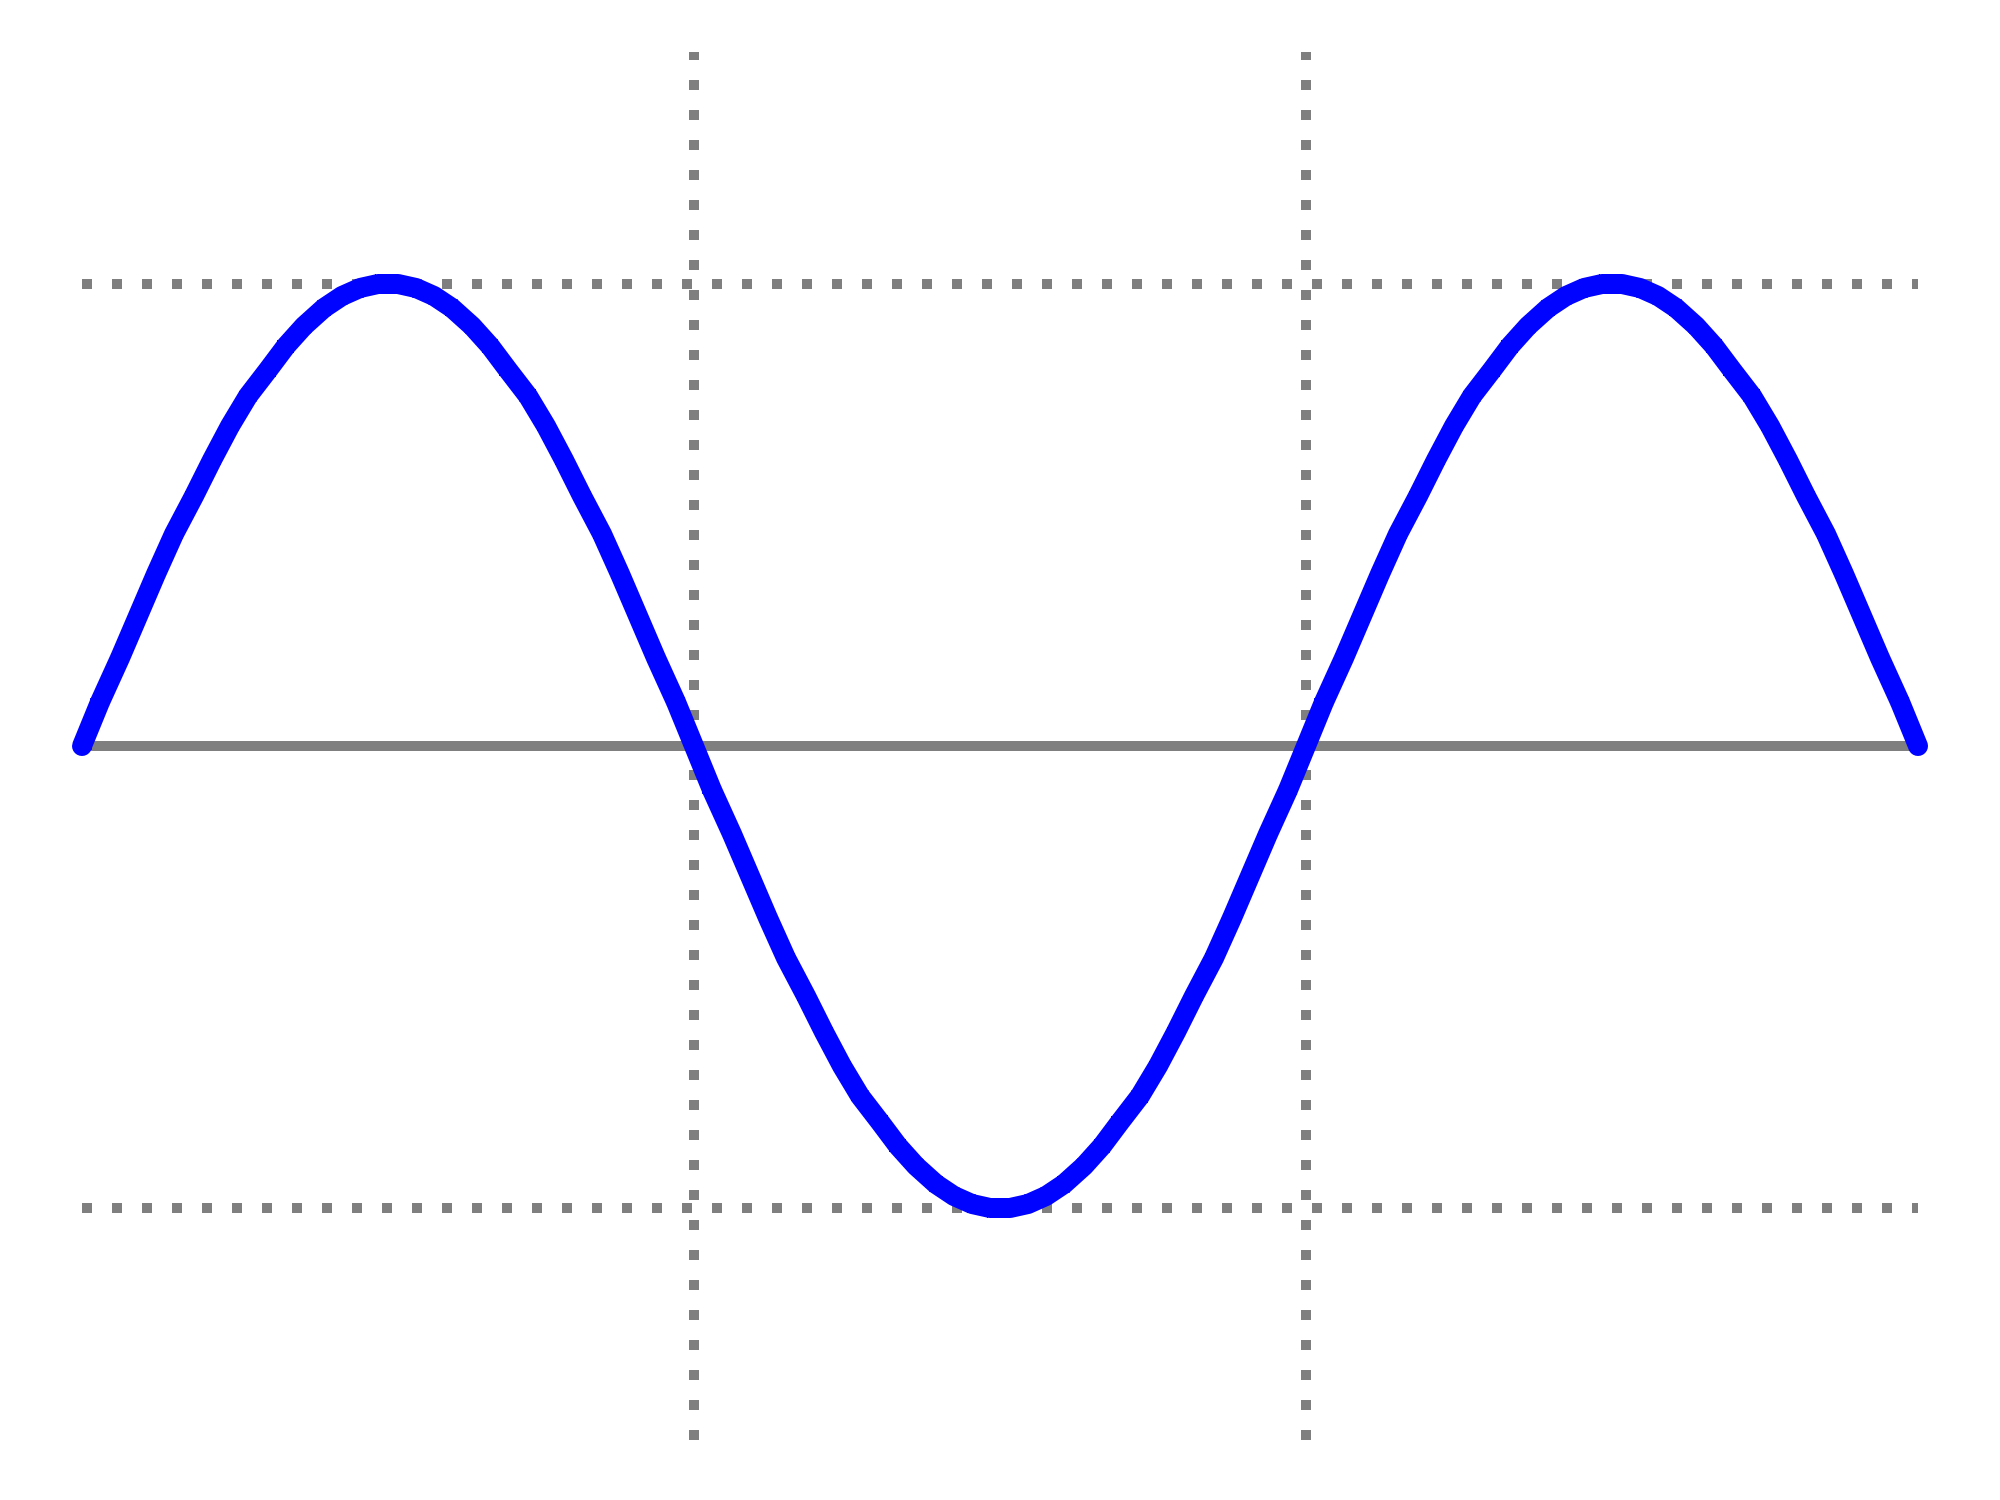
\includegraphics[width=2cm]{images/table_sine_wave.png} &
			$A\cdot\sin(t)$ &
			$\frac{2}{\pi} \approx 0.637$ &
			$\frac{\pi}{2\sqrt{2}} \approx 1.11$ &
			$\frac{1}{\sqrt{2}}\approx 0.707$ &
			$\sqrt{2}\approx 1.414$ &
			$0$ &
			$\frac{A^2}{2}$ &
			$\frac{A^2}{2}$ \\
			\hline	
			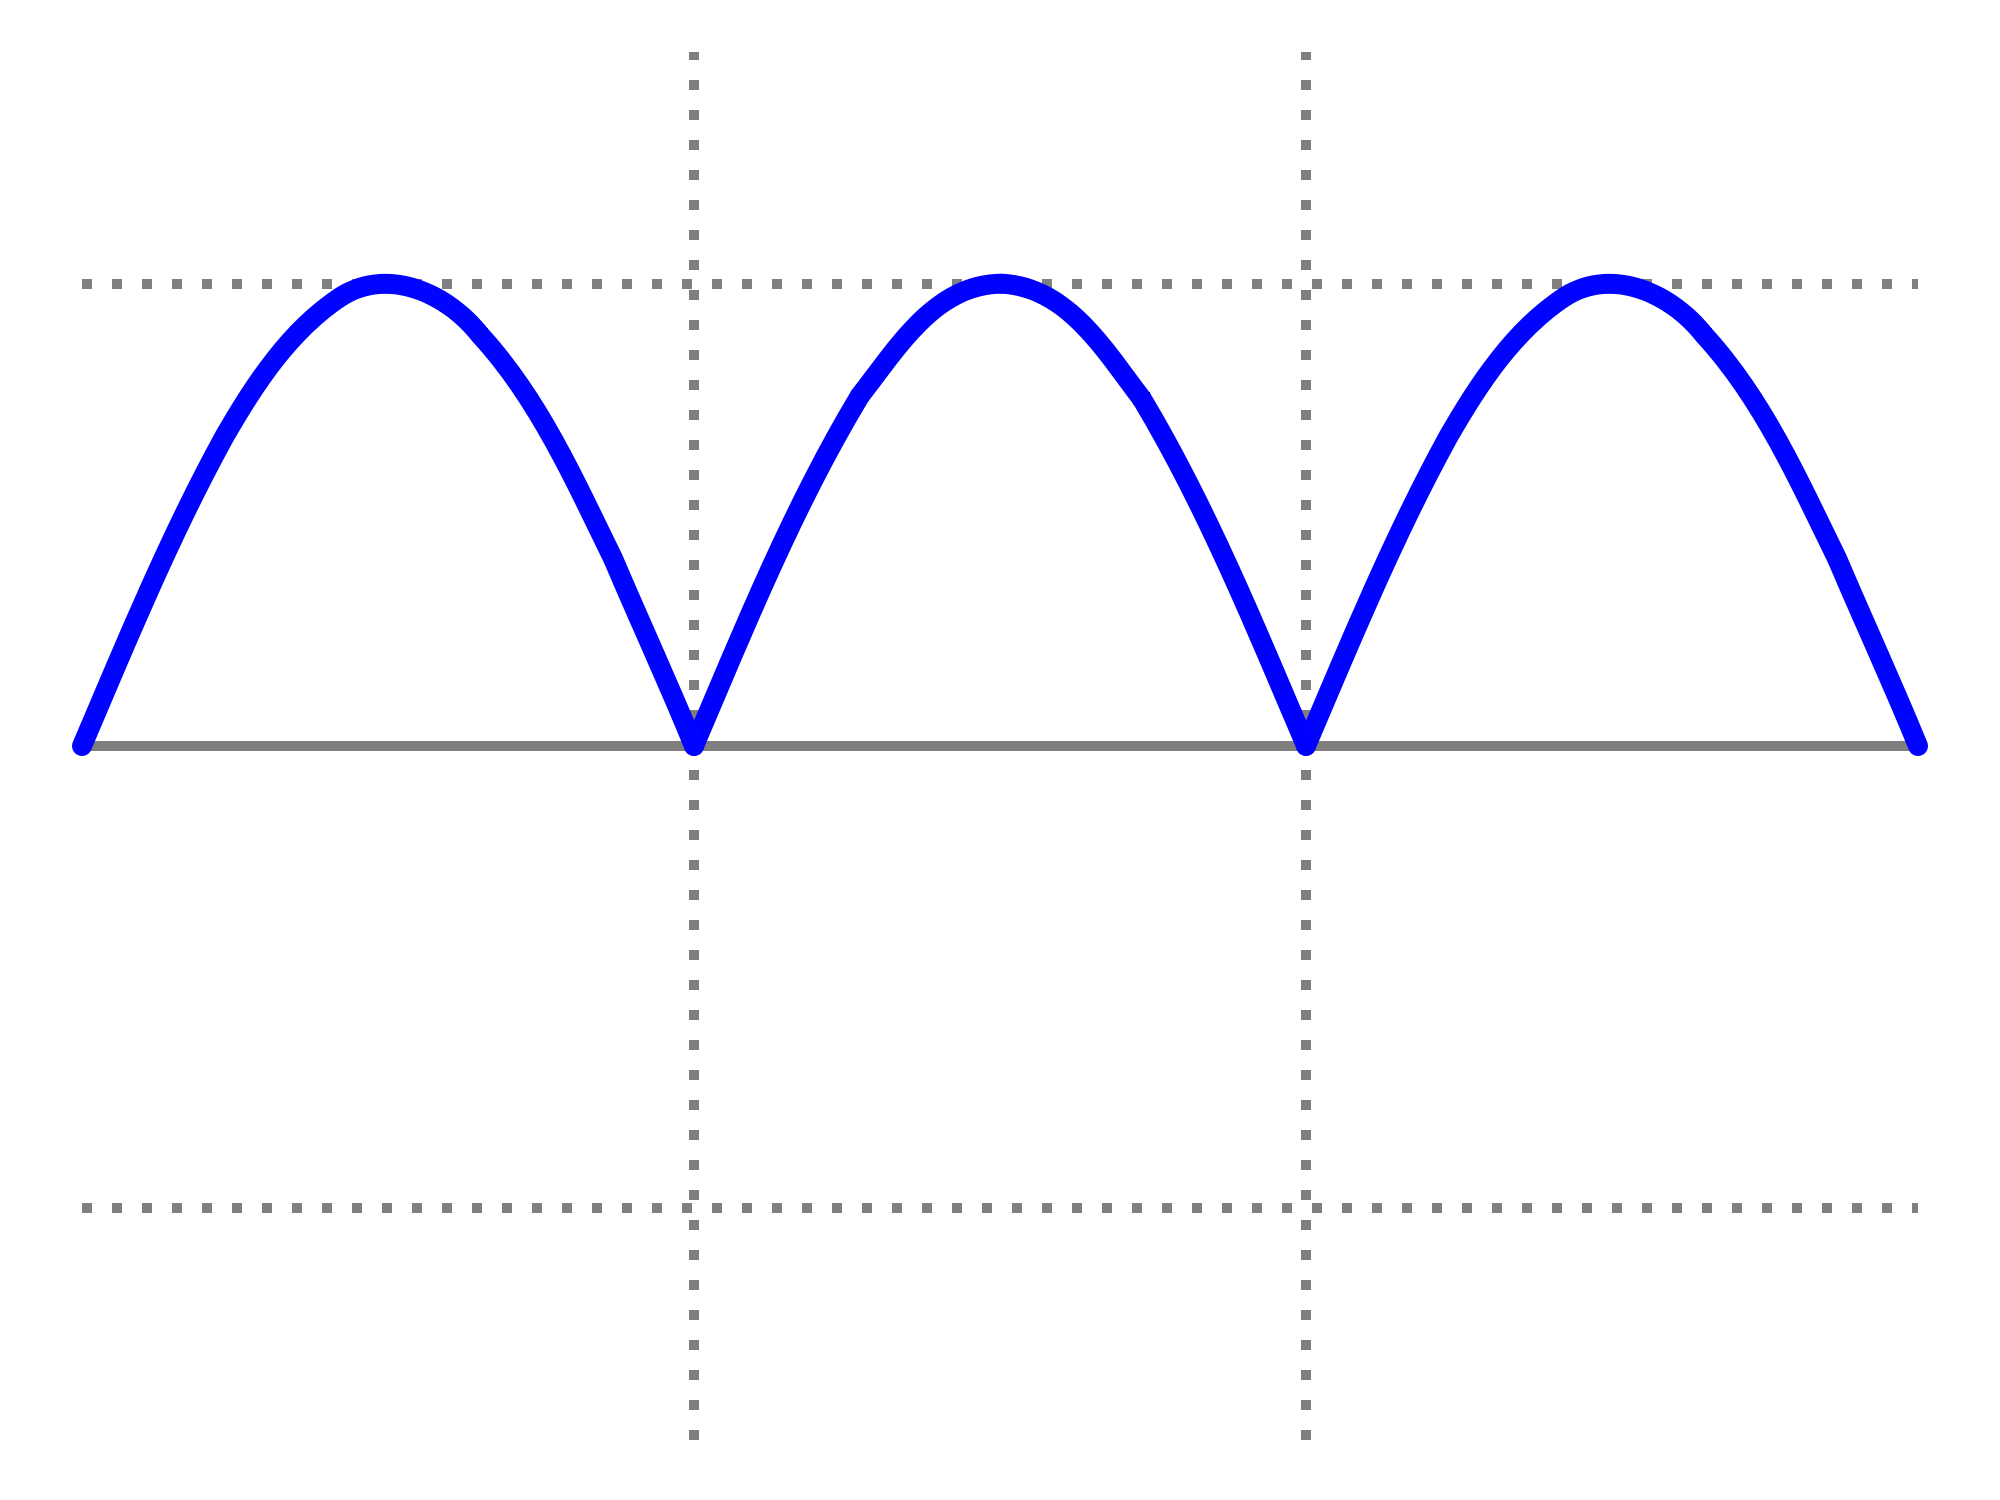
\includegraphics[width=2cm]{images/table_full-wave_rectified_sine.png} &
			$A\cdot|\sin(t)|$ &
			$\frac{2}{\pi} \approx 0.637$ &
			$\frac{\pi}{2\sqrt{2}} \approx 1.11$ &
			$\frac{1}{\sqrt{2}} \approx 0.707$ &
			$\sqrt{2} \approx 1.414$  &
			$\frac{2A}{\pi}$ & $\frac{A^2}{2}$ & $\frac{A^2}{2}-\frac{4A^2}{\pi^2}$
			\\
			\hline
			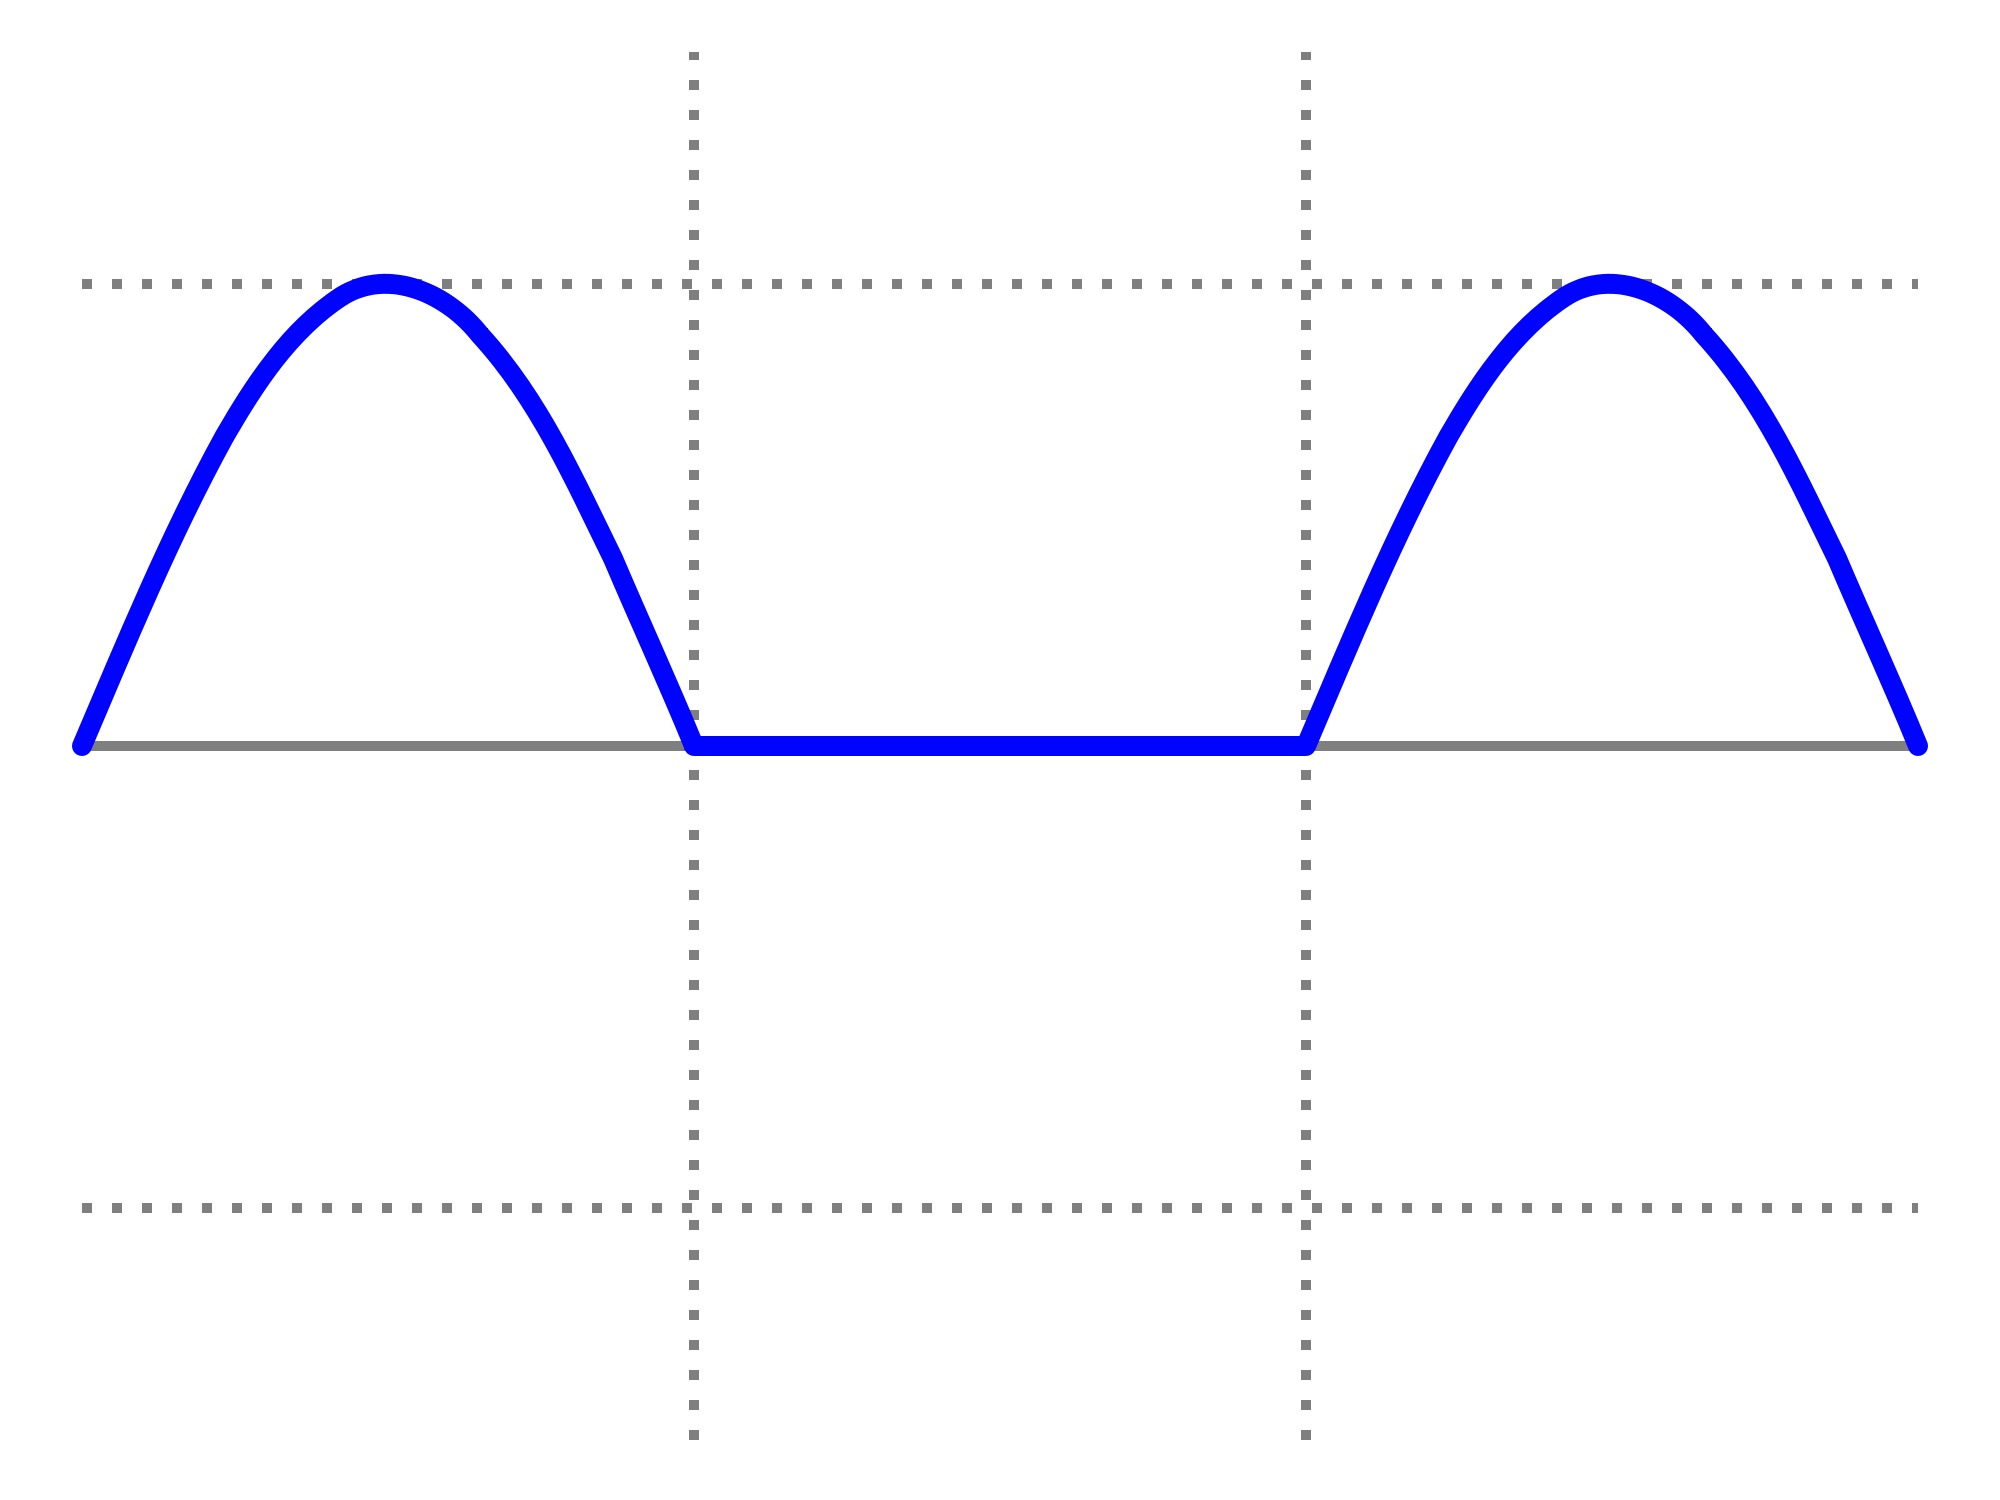
\includegraphics[width=2cm]{images/table_half-wave_rectified_sine.png} &
			$\begin{cases} A\cdot\sin (t) & 0<t<\pi  \\ 0 & \text{True}\end{cases}$ &
			$\frac{1}{\pi}\approx 0.318$ &
			$\frac{\pi}{2}\approx 1.571$ &
			$\frac{1}{2} = 0.5$	&
			2  &
			$\frac{A}{\pi}$ &
			$\frac{A^2}{4}$ & $\frac{A^2}{4}-\frac{A^2}{\pi^2}$
			\\
			\hline
			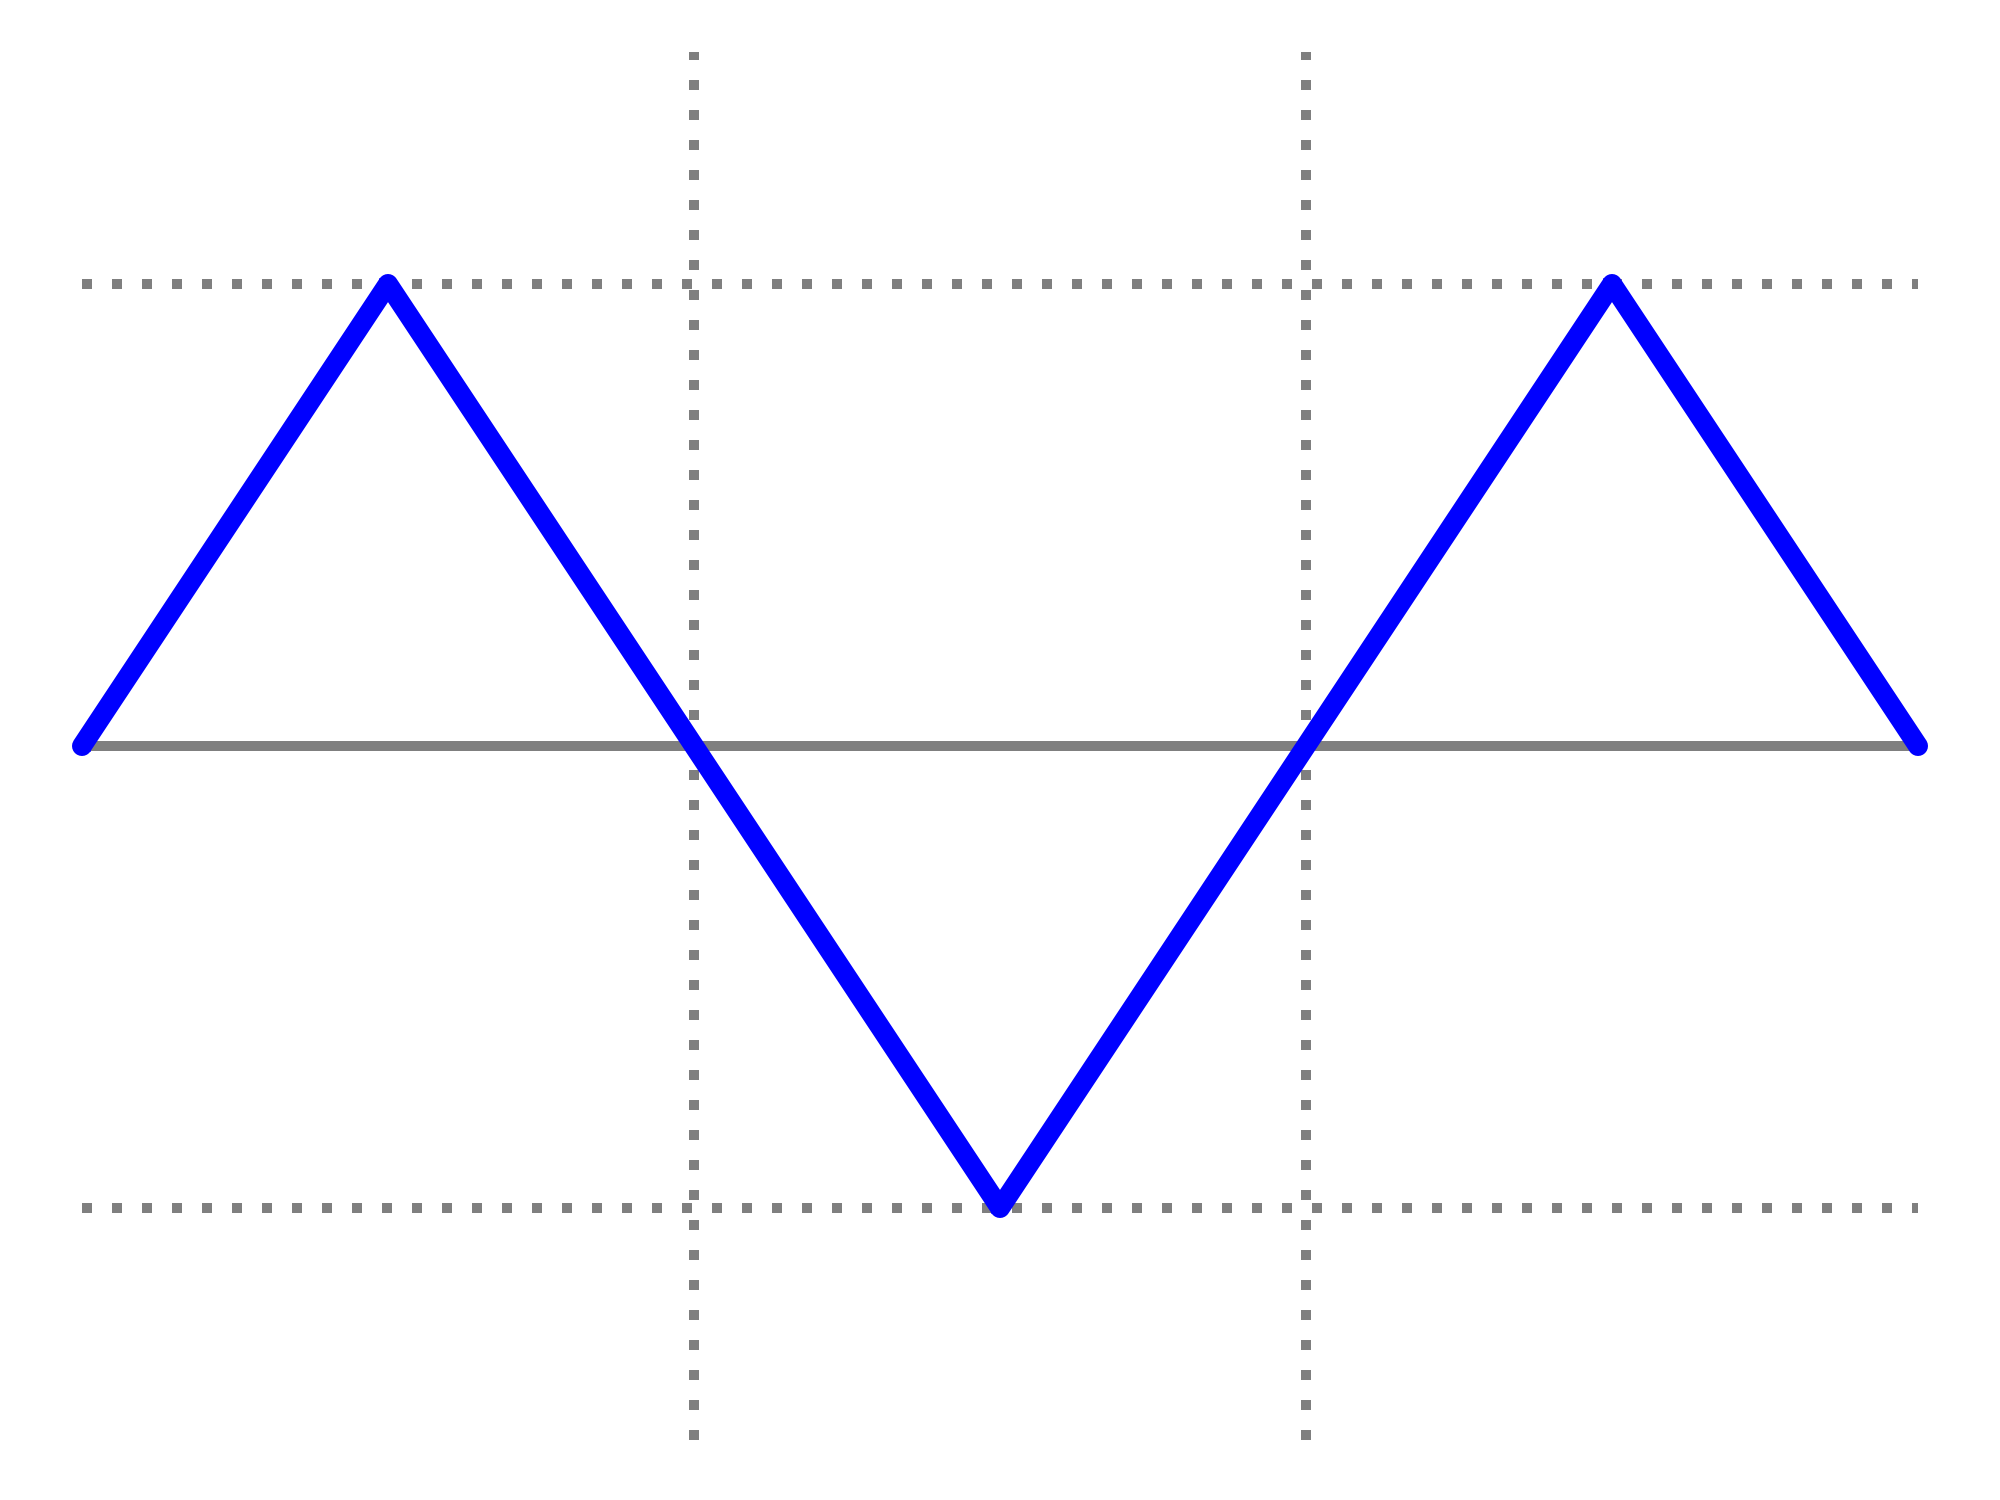
\includegraphics[width=2cm]{images/table_triangle_wave.png} &
			$A\cdot\Lambda(t)$ &
			$\frac{1}{2}= 0.5$ &
			$\frac{2}{\sqrt{3}}\approx 1.155$ &
			$\frac{1}{\sqrt{3}}
			\approx 0.557$ &
			$\sqrt{3} \approx 1.732$ &
			$0$ &
			$\frac{A^2}{3}$ &
			$\frac{A^2}{3}$ \\
			\hline	
			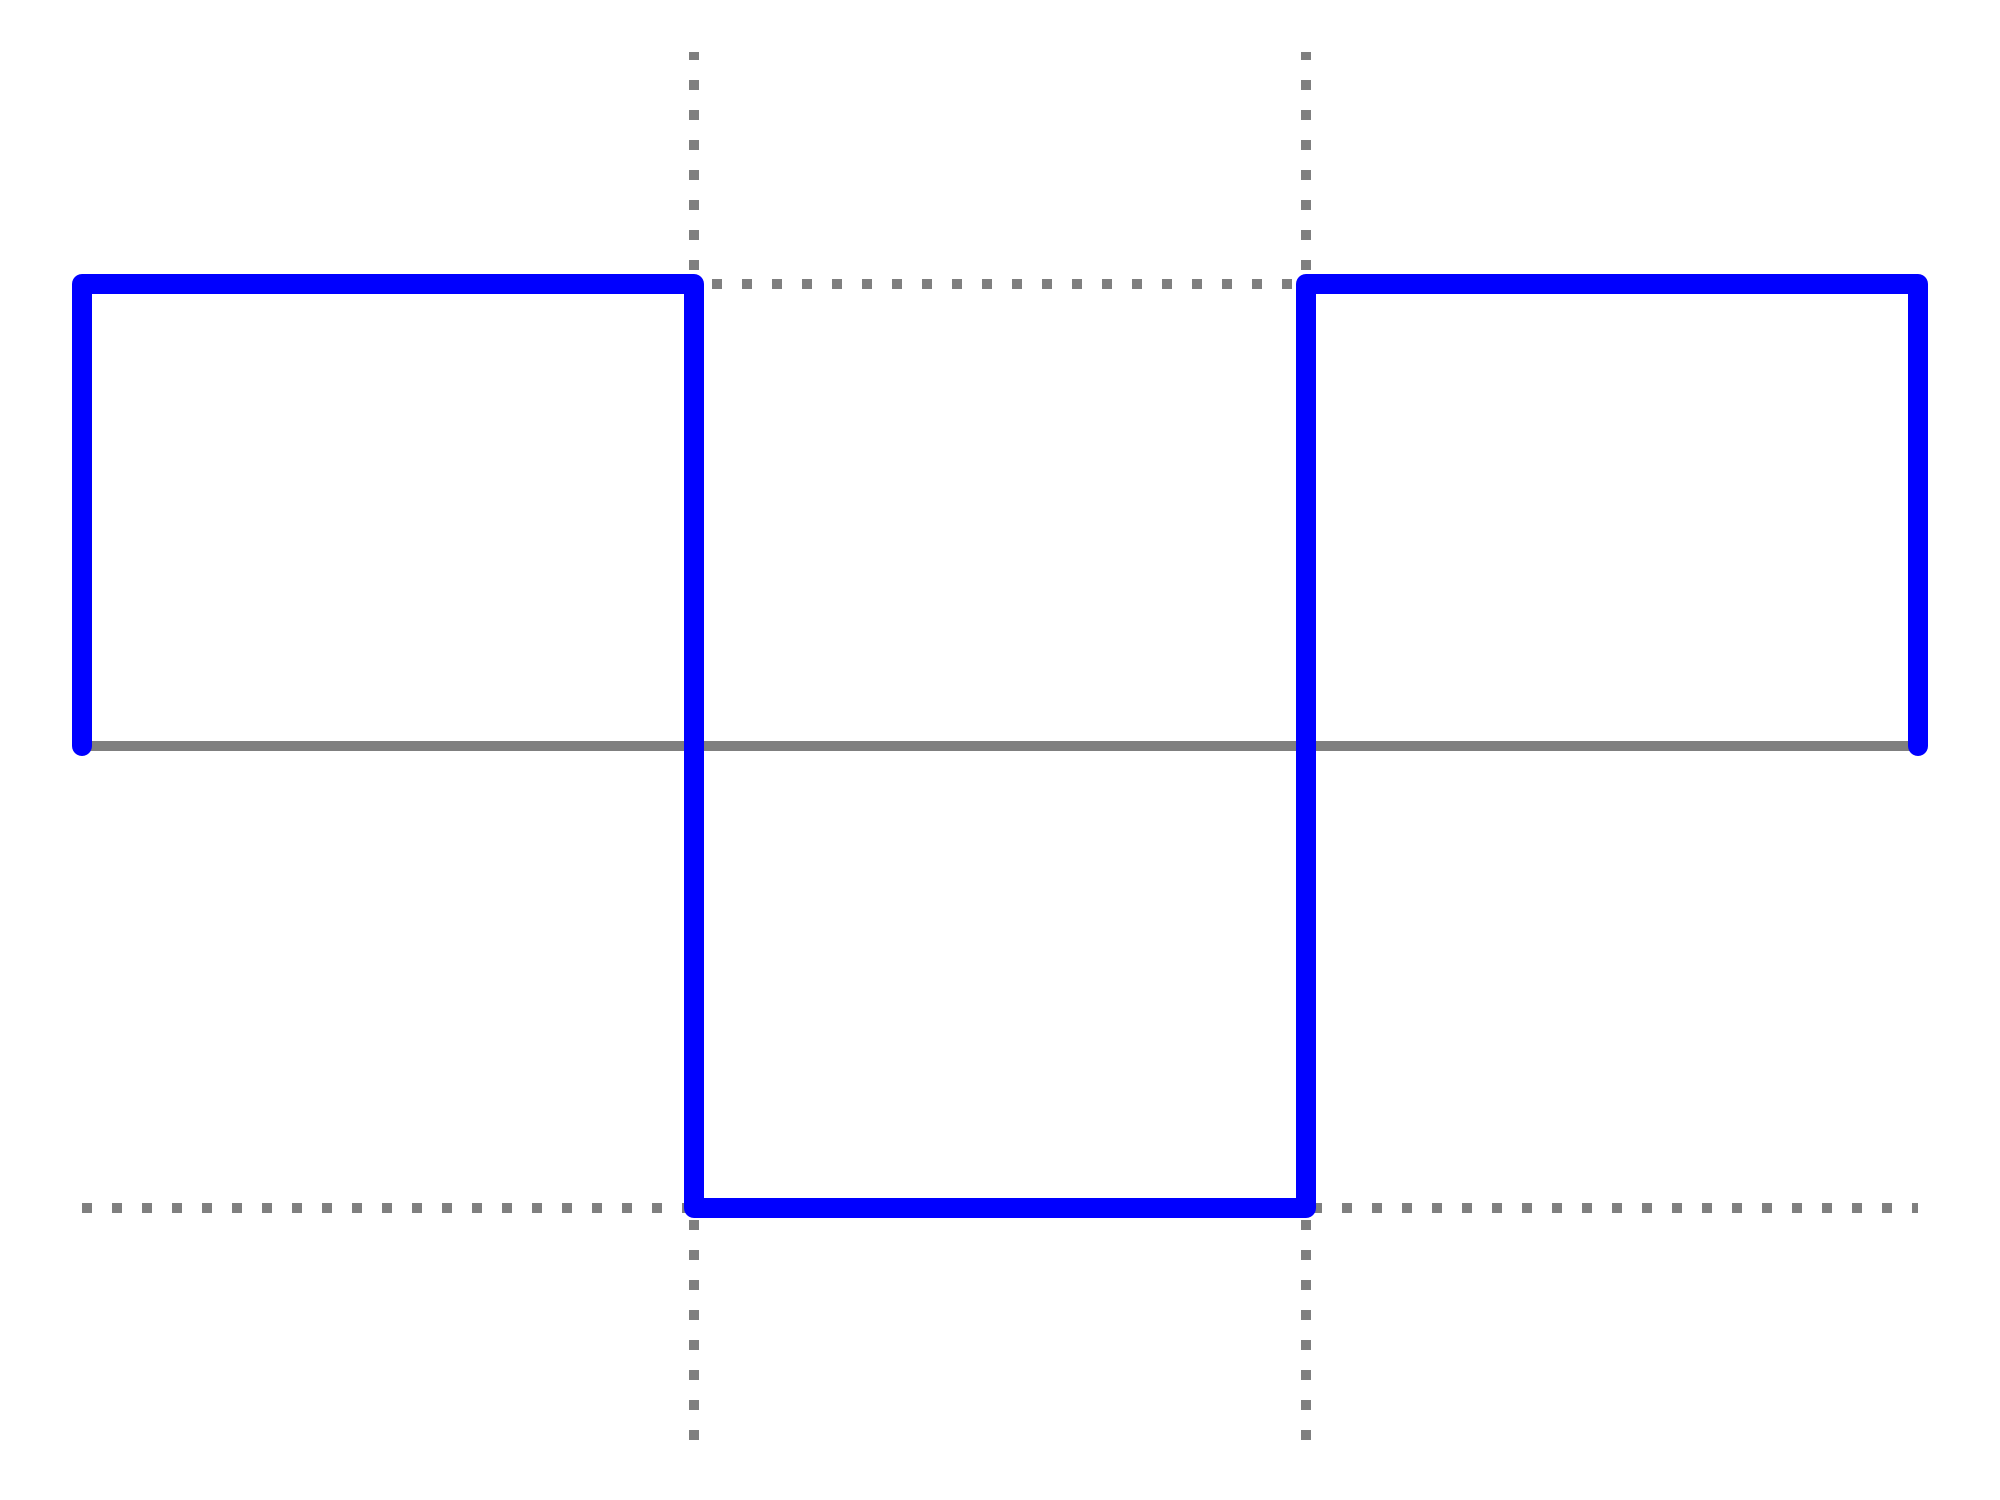
\includegraphics[width=2cm]{images/table_square_wave.png} &
			$\begin{cases} A & 0<x<t \\ 0 & \text{True}\end{cases}$ &
			$1$ &
			$1$ &
			$1$ &
			$1$ &
			$0$ &
			$A^2$ &
			$A^2$ \\
			\hline	
			DC&
			1&
			$1$ &
			$1$ &
			$1$ &
			$1$  &
			-&
			-&
			-\\
			\hline	
			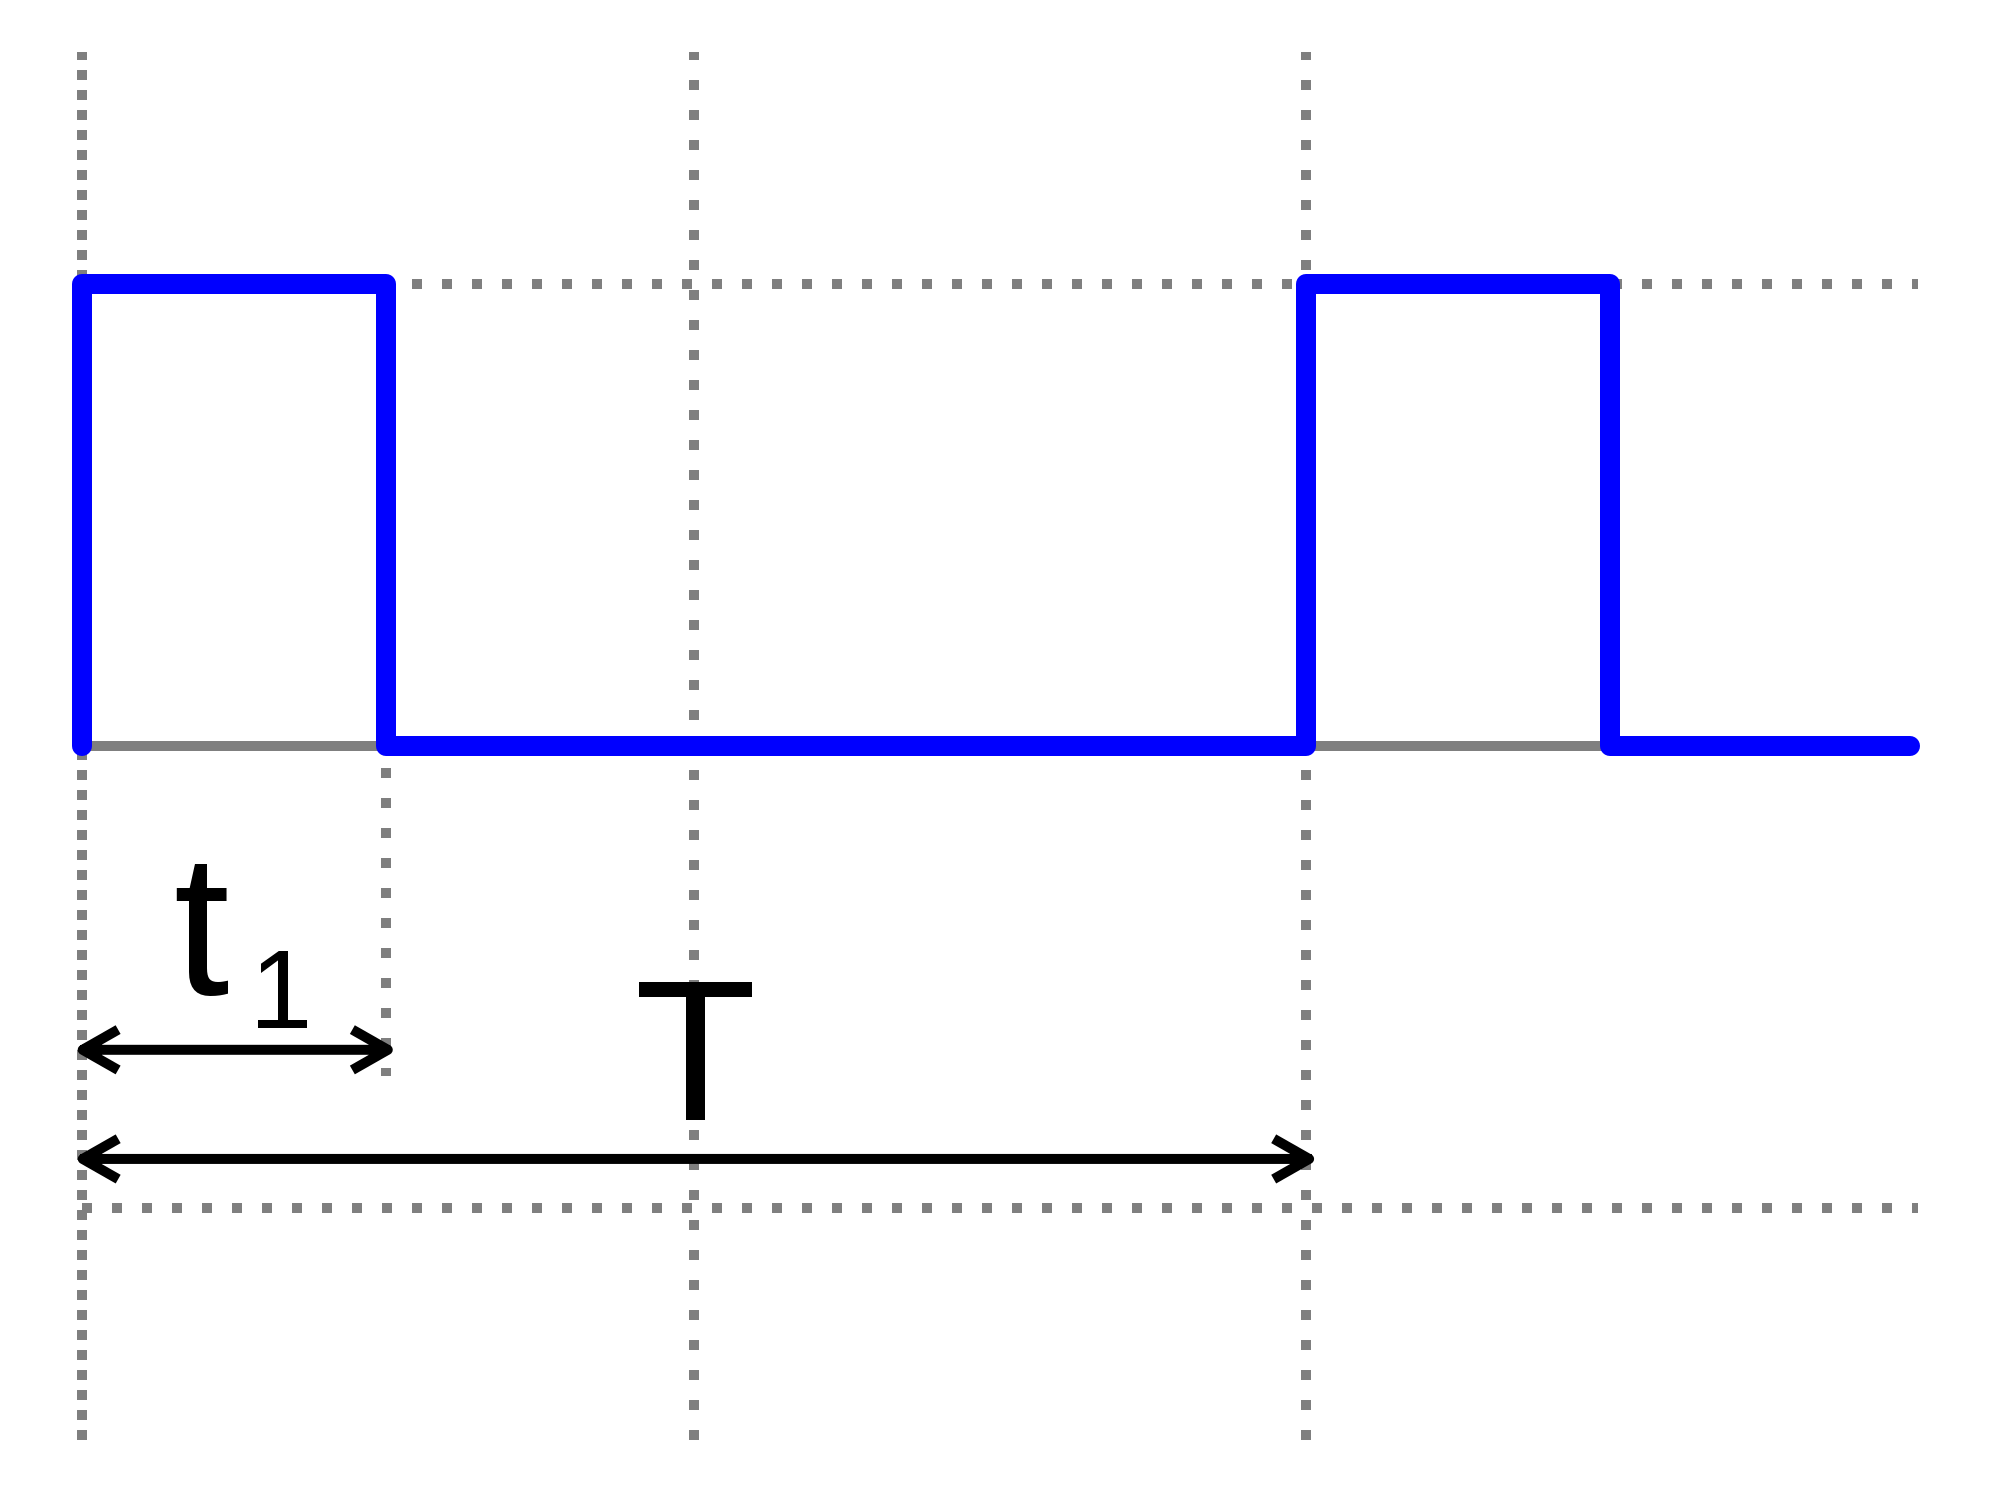
\includegraphics[width=2cm]{images/table_pulse_wide_wave.png} &
			&
			$\frac{t_1}{T}$ & $\sqrt{\frac{T}{t_1}}$ & $\sqrt{\frac{t_1}{T}}$ & $\sqrt{\frac{T}{t_1}}$ &
			$A\frac{t}{T}$ &
			$A^2\frac{t}{T}$ &
			$\frac{A^2t}{T}-\frac{A^2t^2}{T^2}$\\
			\hline
		\end{tabular}
\end{sidewaystable}
\clearpage
\newpage
\section{Linux-Tipps}
%TODO Linux-Befehle etc ergänzen

\end{document}

%TODO Wichtige Sachen aus 4.Semester ergänzen wie Übertragungsfunktion